\documentclass[conference]{IEEEtran}
\usepackage{graphicx}
\usepackage{booktabs}
\usepackage{amsmath,amssymb}
\usepackage{url}
\usepackage[hidelinks]{hyperref}
\usepackage{xcolor}
\usepackage{siunitx}
\usepackage{amsfonts}
\usepackage[export]{adjustbox}
\newcommand{\fitcolumn}[1]{\adjustbox{max width=\columnwidth}{\input{#1}}}
\newcommand{\fitwide}[1]{\adjustbox{max width=\textwidth}{\input{#1}}}
\graphicspath{{../experiments/ndws/}}

% Numbers in the text are macros and tables are generated by `python -m src.evaluation.report_assets`.
% Generated by python -m src.evaluation.report_assets. Do not edit by hand.
\newcommand{\rAblationBaseline}{0.239}
\newcommand{\rAblationNoAugmentation}{0.242}
\newcommand{\rAblationNoDropout}{0.233}
\newcommand{\rAblationNoPrevFireChannel}{0.030}
\newcommand{\rAblationNoRegularisation}{0.231}
\newcommand{\rAblationNoSkipConnections}{0.228}
\newcommand{\rAblationNoTerrainVegetation}{0.228}
\newcommand{\rAblationNoWeatherChannels}{0.227}
\newcommand{\rAblationNoWeightDecay}{0.233}
\newcommand{\rAblationNoWindChannels}{0.233}
\newcommand{\rCnnParameters}{81,097}
\newcommand{\rDevTrain}{12,050}
\newcommand{\rDevVal}{1,466}
\newcommand{\rLocationGroups}{845}
\newcommand{\rNewFireShare}{74}
\newcommand{\rOfficialBestTree}{XGBoost}
\newcommand{\rOfficialCnnSeedMean}{0.255}
\newcommand{\rOfficialCropActiveHybridMinusLightgbmCropDelta}{+0.012}
\newcommand{\rOfficialCropActiveHybridMinusLightgbmCropHigh}{+0.017}
\newcommand{\rOfficialCropActiveHybridMinusLightgbmCropLow}{+0.006}
\newcommand{\rOfficialCropActiveHybridMinusUnetDelta}{+0.005}
\newcommand{\rOfficialCropActiveHybridMinusUnetHigh}{+0.007}
\newcommand{\rOfficialCropActiveHybridMinusUnetLow}{+0.003}
\newcommand{\rOfficialCropActiveLightgbmCropMinusLightgbmFullDelta}{-0.004}
\newcommand{\rOfficialCropActiveLightgbmCropMinusLightgbmFullHigh}{+0.002}
\newcommand{\rOfficialCropActiveLightgbmCropMinusLightgbmFullLow}{-0.011}
\newcommand{\rOfficialCropActiveUnetFeaturesMinusLightgbmCropDelta}{-0.006}
\newcommand{\rOfficialCropActiveUnetFeaturesMinusLightgbmCropHigh}{-0.001}
\newcommand{\rOfficialCropActiveUnetFeaturesMinusLightgbmCropLow}{-0.012}
\newcommand{\rOfficialCropActiveUnetMinusLightgbmCropDelta}{+0.007}
\newcommand{\rOfficialCropActiveUnetMinusLightgbmCropHigh}{+0.014}
\newcommand{\rOfficialCropActiveUnetMinusLightgbmCropLow}{-0.001}
\newcommand{\rOfficialCropCnnCiHigh}{0.307}
\newcommand{\rOfficialCropCnnCiLow}{0.269}
\newcommand{\rOfficialCropCnnLift}{10.0}
\newcommand{\rOfficialCropCnnPr}{0.287}
\newcommand{\rOfficialCropCnnRocAuc}{0.867}
\newcommand{\rOfficialCropFusionTreeCnnCiHigh}{0.314}
\newcommand{\rOfficialCropFusionTreeCnnCiLow}{0.277}
\newcommand{\rOfficialCropFusionTreeCnnLift}{10.3}
\newcommand{\rOfficialCropFusionTreeCnnPr}{0.294}
\newcommand{\rOfficialCropFusionTreeCnnRocAuc}{0.876}
\newcommand{\rOfficialCropFusionTreeOnlyCiHigh}{0.310}
\newcommand{\rOfficialCropFusionTreeOnlyCiLow}{0.273}
\newcommand{\rOfficialCropFusionTreeOnlyLift}{10.1}
\newcommand{\rOfficialCropFusionTreeOnlyPr}{0.290}
\newcommand{\rOfficialCropFusionTreeOnlyRocAuc}{0.871}
\newcommand{\rOfficialCropFusionTreeUnetCiHigh}{0.321}
\newcommand{\rOfficialCropFusionTreeUnetCiLow}{0.283}
\newcommand{\rOfficialCropFusionTreeUnetFeaturesCiHigh}{0.314}
\newcommand{\rOfficialCropFusionTreeUnetFeaturesCiLow}{0.276}
\newcommand{\rOfficialCropFusionTreeUnetFeaturesLift}{10.3}
\newcommand{\rOfficialCropFusionTreeUnetFeaturesPr}{0.293}
\newcommand{\rOfficialCropFusionTreeUnetFeaturesRocAuc}{0.872}
\newcommand{\rOfficialCropFusionTreeUnetLift}{10.5}
\newcommand{\rOfficialCropFusionTreeUnetPr}{0.301}
\newcommand{\rOfficialCropFusionTreeUnetRocAuc}{0.878}
\newcommand{\rOfficialCropFusionUnetOnlyCiHigh}{0.316}
\newcommand{\rOfficialCropFusionUnetOnlyCiLow}{0.278}
\newcommand{\rOfficialCropFusionUnetOnlyLift}{10.4}
\newcommand{\rOfficialCropFusionUnetOnlyPr}{0.297}
\newcommand{\rOfficialCropFusionUnetOnlyRocAuc}{0.876}
\newcommand{\rOfficialCropHybridCiHigh}{0.321}
\newcommand{\rOfficialCropHybridCiLow}{0.283}
\newcommand{\rOfficialCropHybridLift}{10.5}
\newcommand{\rOfficialCropHybridPr}{0.301}
\newcommand{\rOfficialCropHybridRocAuc}{0.878}
\newcommand{\rOfficialCropLightgbmCropCiHigh}{0.310}
\newcommand{\rOfficialCropLightgbmCropCiLow}{0.273}
\newcommand{\rOfficialCropLightgbmCropLift}{10.1}
\newcommand{\rOfficialCropLightgbmCropPr}{0.290}
\newcommand{\rOfficialCropLightgbmCropRocAuc}{0.871}
\newcommand{\rOfficialCropLightgbmFullCiHigh}{0.316}
\newcommand{\rOfficialCropLightgbmFullCiLow}{0.274}
\newcommand{\rOfficialCropLightgbmFullLift}{10.3}
\newcommand{\rOfficialCropLightgbmFullPr}{0.293}
\newcommand{\rOfficialCropLightgbmFullRocAuc}{0.876}
\newcommand{\rOfficialCropPositionPriorCiHigh}{0.036}
\newcommand{\rOfficialCropPositionPriorCiLow}{0.030}
\newcommand{\rOfficialCropPositionPriorLift}{1.1}
\newcommand{\rOfficialCropPositionPriorPr}{0.032}
\newcommand{\rOfficialCropPositionPriorRocAuc}{0.549}
\newcommand{\rOfficialCropTransitionHybridMinusLightgbmCropDelta}{+0.016}
\newcommand{\rOfficialCropTransitionHybridMinusLightgbmCropHigh}{+0.020}
\newcommand{\rOfficialCropTransitionHybridMinusLightgbmCropLow}{+0.010}
\newcommand{\rOfficialCropTransitionHybridMinusUnetDelta}{+0.003}
\newcommand{\rOfficialCropTransitionHybridMinusUnetHigh}{+0.005}
\newcommand{\rOfficialCropTransitionHybridMinusUnetLow}{+0.001}
\newcommand{\rOfficialCropTransitionLightgbmCropMinusLightgbmFullDelta}{+0.001}
\newcommand{\rOfficialCropTransitionLightgbmCropMinusLightgbmFullHigh}{+0.006}
\newcommand{\rOfficialCropTransitionLightgbmCropMinusLightgbmFullLow}{-0.003}
\newcommand{\rOfficialCropTransitionUnetFeaturesMinusLightgbmCropDelta}{-0.005}
\newcommand{\rOfficialCropTransitionUnetFeaturesMinusLightgbmCropHigh}{+0.000}
\newcommand{\rOfficialCropTransitionUnetFeaturesMinusLightgbmCropLow}{-0.010}
\newcommand{\rOfficialCropTransitionUnetMinusLightgbmCropDelta}{+0.012}
\newcommand{\rOfficialCropTransitionUnetMinusLightgbmCropHigh}{+0.019}
\newcommand{\rOfficialCropTransitionUnetMinusLightgbmCropLow}{+0.006}
\newcommand{\rOfficialCropUnetCiHigh}{0.316}
\newcommand{\rOfficialCropUnetCiLow}{0.278}
\newcommand{\rOfficialCropUnetFeaturesCiHigh}{0.304}
\newcommand{\rOfficialCropUnetFeaturesCiLow}{0.265}
\newcommand{\rOfficialCropUnetFeaturesLift}{9.9}
\newcommand{\rOfficialCropUnetFeaturesPr}{0.284}
\newcommand{\rOfficialCropUnetFeaturesRocAuc}{0.853}
\newcommand{\rOfficialCropUnetLift}{10.4}
\newcommand{\rOfficialCropUnetPr}{0.297}
\newcommand{\rOfficialCropUnetRocAuc}{0.876}
\newcommand{\rOfficialFullActiveCnnMinusXgboostDelta}{-0.009}
\newcommand{\rOfficialFullActiveCnnMinusXgboostHigh}{-0.003}
\newcommand{\rOfficialFullActiveCnnMinusXgboostLow}{-0.014}
\newcommand{\rOfficialFullActiveHybridMinusUnetDelta}{+0.003}
\newcommand{\rOfficialFullActiveHybridMinusUnetHigh}{+0.008}
\newcommand{\rOfficialFullActiveHybridMinusUnetLow}{-0.002}
\newcommand{\rOfficialFullActiveHybridMinusXgboostDelta}{-0.006}
\newcommand{\rOfficialFullActiveHybridMinusXgboostHigh}{-0.002}
\newcommand{\rOfficialFullActiveHybridMinusXgboostLow}{-0.010}
\newcommand{\rOfficialFullActiveLightgbmMinusLogisticRegressionDelta}{+0.032}
\newcommand{\rOfficialFullActiveLightgbmMinusLogisticRegressionHigh}{+0.040}
\newcommand{\rOfficialFullActiveLightgbmMinusLogisticRegressionLow}{+0.025}
\newcommand{\rOfficialFullActiveUnetFeaturesMinusUnetDelta}{-0.002}
\newcommand{\rOfficialFullActiveUnetFeaturesMinusUnetHigh}{+0.003}
\newcommand{\rOfficialFullActiveUnetFeaturesMinusUnetLow}{-0.008}
\newcommand{\rOfficialFullActiveUnetFeaturesMinusXgboostDelta}{-0.011}
\newcommand{\rOfficialFullActiveUnetFeaturesMinusXgboostHigh}{-0.007}
\newcommand{\rOfficialFullActiveUnetFeaturesMinusXgboostLow}{-0.015}
\newcommand{\rOfficialFullActiveUnetFullpatchMinusUnetDelta}{+0.084}
\newcommand{\rOfficialFullActiveUnetFullpatchMinusUnetHigh}{+0.093}
\newcommand{\rOfficialFullActiveUnetFullpatchMinusUnetLow}{+0.076}
\newcommand{\rOfficialFullActiveUnetMinusCnnDelta}{+0.001}
\newcommand{\rOfficialFullActiveUnetMinusCnnHigh}{+0.005}
\newcommand{\rOfficialFullActiveUnetMinusCnnLow}{-0.004}
\newcommand{\rOfficialFullActiveUnetMinusXgboostDelta}{-0.008}
\newcommand{\rOfficialFullActiveUnetMinusXgboostHigh}{-0.002}
\newcommand{\rOfficialFullActiveUnetMinusXgboostLow}{-0.014}
\newcommand{\rOfficialFullActiveXgboostMinusLightgbmDelta}{+0.002}
\newcommand{\rOfficialFullActiveXgboostMinusLightgbmHigh}{+0.006}
\newcommand{\rOfficialFullActiveXgboostMinusLightgbmLow}{-0.001}
\newcommand{\rOfficialFullCentrePriorCiHigh}{0.142}
\newcommand{\rOfficialFullCentrePriorCiLow}{0.129}
\newcommand{\rOfficialFullCentrePriorLift}{10.8}
\newcommand{\rOfficialFullCentrePriorPr}{0.135}
\newcommand{\rOfficialFullCentrePriorRocAuc}{0.798}
\newcommand{\rOfficialFullCnnCiHigh}{0.272}
\newcommand{\rOfficialFullCnnCiLow}{0.240}
\newcommand{\rOfficialFullCnnF}{0.332}
\newcommand{\rOfficialFullCnnLift}{20.4}
\newcommand{\rOfficialFullCnnPr}{0.256}
\newcommand{\rOfficialFullCnnPrecision}{0.242}
\newcommand{\rOfficialFullCnnRecall}{0.529}
\newcommand{\rOfficialFullCnnRocAuc}{0.897}
\newcommand{\rOfficialFullDummyCiHigh}{0.014}
\newcommand{\rOfficialFullDummyCiLow}{0.012}
\newcommand{\rOfficialFullDummyF}{0.025}
\newcommand{\rOfficialFullDummyLift}{1.0}
\newcommand{\rOfficialFullDummyPr}{0.013}
\newcommand{\rOfficialFullDummyPrecision}{0.013}
\newcommand{\rOfficialFullDummyRecall}{1.000}
\newcommand{\rOfficialFullDummyRocAuc}{0.500}
\newcommand{\rOfficialFullFusionTreeCnnCiHigh}{0.284}
\newcommand{\rOfficialFullFusionTreeCnnCiLow}{0.250}
\newcommand{\rOfficialFullFusionTreeCnnF}{0.328}
\newcommand{\rOfficialFullFusionTreeCnnLift}{21.3}
\newcommand{\rOfficialFullFusionTreeCnnPr}{0.266}
\newcommand{\rOfficialFullFusionTreeCnnPrecision}{0.236}
\newcommand{\rOfficialFullFusionTreeCnnRecall}{0.540}
\newcommand{\rOfficialFullFusionTreeCnnRocAuc}{0.912}
\newcommand{\rOfficialFullFusionTreeOnlyCiHigh}{0.283}
\newcommand{\rOfficialFullFusionTreeOnlyCiLow}{0.248}
\newcommand{\rOfficialFullFusionTreeOnlyF}{0.327}
\newcommand{\rOfficialFullFusionTreeOnlyLift}{21.1}
\newcommand{\rOfficialFullFusionTreeOnlyPr}{0.265}
\newcommand{\rOfficialFullFusionTreeOnlyPrecision}{0.234}
\newcommand{\rOfficialFullFusionTreeOnlyRecall}{0.540}
\newcommand{\rOfficialFullFusionTreeOnlyRocAuc}{0.911}
\newcommand{\rOfficialFullFusionTreeUnetCiHigh}{0.286}
\newcommand{\rOfficialFullFusionTreeUnetCiLow}{0.254}
\newcommand{\rOfficialFullFusionTreeUnetF}{0.342}
\newcommand{\rOfficialFullFusionTreeUnetFeaturesCiHigh}{0.276}
\newcommand{\rOfficialFullFusionTreeUnetFeaturesCiLow}{0.244}
\newcommand{\rOfficialFullFusionTreeUnetFeaturesF}{0.340}
\newcommand{\rOfficialFullFusionTreeUnetFeaturesLift}{20.7}
\newcommand{\rOfficialFullFusionTreeUnetFeaturesPr}{0.259}
\newcommand{\rOfficialFullFusionTreeUnetFeaturesPrecision}{0.254}
\newcommand{\rOfficialFullFusionTreeUnetFeaturesRecall}{0.514}
\newcommand{\rOfficialFullFusionTreeUnetFeaturesRocAuc}{0.917}
\newcommand{\rOfficialFullFusionTreeUnetLift}{21.5}
\newcommand{\rOfficialFullFusionTreeUnetPr}{0.270}
\newcommand{\rOfficialFullFusionTreeUnetPrecision}{0.253}
\newcommand{\rOfficialFullFusionTreeUnetRecall}{0.528}
\newcommand{\rOfficialFullFusionTreeUnetRocAuc}{0.908}
\newcommand{\rOfficialFullFusionUnetOnlyCiHigh}{0.272}
\newcommand{\rOfficialFullFusionUnetOnlyCiLow}{0.242}
\newcommand{\rOfficialFullFusionUnetOnlyF}{0.349}
\newcommand{\rOfficialFullFusionUnetOnlyLift}{20.5}
\newcommand{\rOfficialFullFusionUnetOnlyPr}{0.257}
\newcommand{\rOfficialFullFusionUnetOnlyPrecision}{0.269}
\newcommand{\rOfficialFullFusionUnetOnlyRecall}{0.495}
\newcommand{\rOfficialFullFusionUnetOnlyRocAuc}{0.892}
\newcommand{\rOfficialFullHybridCiHigh}{0.276}
\newcommand{\rOfficialFullHybridCiLow}{0.244}
\newcommand{\rOfficialFullHybridF}{0.340}
\newcommand{\rOfficialFullHybridLift}{20.7}
\newcommand{\rOfficialFullHybridPr}{0.259}
\newcommand{\rOfficialFullHybridPrecision}{0.254}
\newcommand{\rOfficialFullHybridRecall}{0.514}
\newcommand{\rOfficialFullHybridRocAuc}{0.917}
\newcommand{\rOfficialFullLightgbmCiHigh}{0.281}
\newcommand{\rOfficialFullLightgbmCiLow}{0.246}
\newcommand{\rOfficialFullLightgbmF}{0.334}
\newcommand{\rOfficialFullLightgbmLift}{21.0}
\newcommand{\rOfficialFullLightgbmPr}{0.263}
\newcommand{\rOfficialFullLightgbmPrecision}{0.245}
\newcommand{\rOfficialFullLightgbmRecall}{0.525}
\newcommand{\rOfficialFullLightgbmRocAuc}{0.905}
\newcommand{\rOfficialFullLogisticRegressionCiHigh}{0.249}
\newcommand{\rOfficialFullLogisticRegressionCiLow}{0.213}
\newcommand{\rOfficialFullLogisticRegressionF}{0.327}
\newcommand{\rOfficialFullLogisticRegressionLift}{18.4}
\newcommand{\rOfficialFullLogisticRegressionPr}{0.230}
\newcommand{\rOfficialFullLogisticRegressionPrecision}{0.246}
\newcommand{\rOfficialFullLogisticRegressionRecall}{0.487}
\newcommand{\rOfficialFullLogisticRegressionRocAuc}{0.903}
\newcommand{\rOfficialFullNeighbourhoodPersistCiHigh}{0.191}
\newcommand{\rOfficialFullNeighbourhoodPersistCiLow}{0.157}
\newcommand{\rOfficialFullNeighbourhoodPersistF}{0.328}
\newcommand{\rOfficialFullNeighbourhoodPersistLift}{13.8}
\newcommand{\rOfficialFullNeighbourhoodPersistPr}{0.173}
\newcommand{\rOfficialFullNeighbourhoodPersistPrecision}{0.251}
\newcommand{\rOfficialFullNeighbourhoodPersistRecall}{0.473}
\newcommand{\rOfficialFullNeighbourhoodPersistRocAuc}{0.729}
\newcommand{\rOfficialFullPersistenceCiHigh}{0.118}
\newcommand{\rOfficialFullPersistenceCiLow}{0.097}
\newcommand{\rOfficialFullPersistenceF}{0.309}
\newcommand{\rOfficialFullPersistenceLift}{8.5}
\newcommand{\rOfficialFullPersistencePr}{0.107}
\newcommand{\rOfficialFullPersistencePrecision}{0.357}
\newcommand{\rOfficialFullPersistenceRecall}{0.273}
\newcommand{\rOfficialFullPersistenceRocAuc}{0.633}
\newcommand{\rOfficialFullRandomForestCiHigh}{0.282}
\newcommand{\rOfficialFullRandomForestCiLow}{0.248}
\newcommand{\rOfficialFullRandomForestF}{0.343}
\newcommand{\rOfficialFullRandomForestLift}{21.1}
\newcommand{\rOfficialFullRandomForestPr}{0.265}
\newcommand{\rOfficialFullRandomForestPrecision}{0.261}
\newcommand{\rOfficialFullRandomForestRecall}{0.498}
\newcommand{\rOfficialFullRandomForestRocAuc}{0.901}
\newcommand{\rOfficialFullTransitionCnnMinusXgboostDelta}{+0.002}
\newcommand{\rOfficialFullTransitionCnnMinusXgboostHigh}{+0.006}
\newcommand{\rOfficialFullTransitionCnnMinusXgboostLow}{-0.001}
\newcommand{\rOfficialFullTransitionHybridMinusUnetDelta}{-0.004}
\newcommand{\rOfficialFullTransitionHybridMinusUnetHigh}{+0.000}
\newcommand{\rOfficialFullTransitionHybridMinusUnetLow}{-0.008}
\newcommand{\rOfficialFullTransitionHybridMinusXgboostDelta}{+0.001}
\newcommand{\rOfficialFullTransitionHybridMinusXgboostHigh}{+0.004}
\newcommand{\rOfficialFullTransitionHybridMinusXgboostLow}{-0.002}
\newcommand{\rOfficialFullTransitionLightgbmMinusLogisticRegressionDelta}{+0.015}
\newcommand{\rOfficialFullTransitionLightgbmMinusLogisticRegressionHigh}{+0.019}
\newcommand{\rOfficialFullTransitionLightgbmMinusLogisticRegressionLow}{+0.012}
\newcommand{\rOfficialFullTransitionUnetFeaturesMinusUnetDelta}{-0.007}
\newcommand{\rOfficialFullTransitionUnetFeaturesMinusUnetHigh}{-0.003}
\newcommand{\rOfficialFullTransitionUnetFeaturesMinusUnetLow}{-0.011}
\newcommand{\rOfficialFullTransitionUnetFeaturesMinusXgboostDelta}{-0.002}
\newcommand{\rOfficialFullTransitionUnetFeaturesMinusXgboostHigh}{+0.001}
\newcommand{\rOfficialFullTransitionUnetFeaturesMinusXgboostLow}{-0.005}
\newcommand{\rOfficialFullTransitionUnetFullpatchMinusUnetDelta}{+0.101}
\newcommand{\rOfficialFullTransitionUnetFullpatchMinusUnetHigh}{+0.111}
\newcommand{\rOfficialFullTransitionUnetFullpatchMinusUnetLow}{+0.091}
\newcommand{\rOfficialFullTransitionUnetMinusCnnDelta}{+0.002}
\newcommand{\rOfficialFullTransitionUnetMinusCnnHigh}{+0.006}
\newcommand{\rOfficialFullTransitionUnetMinusCnnLow}{-0.001}
\newcommand{\rOfficialFullTransitionUnetMinusXgboostDelta}{+0.005}
\newcommand{\rOfficialFullTransitionUnetMinusXgboostHigh}{+0.009}
\newcommand{\rOfficialFullTransitionUnetMinusXgboostLow}{+0.000}
\newcommand{\rOfficialFullTransitionXgboostMinusLightgbmDelta}{+0.003}
\newcommand{\rOfficialFullTransitionXgboostMinusLightgbmHigh}{+0.005}
\newcommand{\rOfficialFullTransitionXgboostMinusLightgbmLow}{+0.000}
\newcommand{\rOfficialFullUnetCiHigh}{0.272}
\newcommand{\rOfficialFullUnetCiLow}{0.242}
\newcommand{\rOfficialFullUnetF}{0.351}
\newcommand{\rOfficialFullUnetFeaturesCiHigh}{0.270}
\newcommand{\rOfficialFullUnetFeaturesCiLow}{0.239}
\newcommand{\rOfficialFullUnetFeaturesF}{0.340}
\newcommand{\rOfficialFullUnetFeaturesLift}{20.3}
\newcommand{\rOfficialFullUnetFeaturesPr}{0.254}
\newcommand{\rOfficialFullUnetFeaturesPrecision}{0.258}
\newcommand{\rOfficialFullUnetFeaturesRecall}{0.500}
\newcommand{\rOfficialFullUnetFeaturesRocAuc}{0.915}
\newcommand{\rOfficialFullUnetFullpatchCiHigh}{0.356}
\newcommand{\rOfficialFullUnetFullpatchCiLow}{0.324}
\newcommand{\rOfficialFullUnetFullpatchF}{0.400}
\newcommand{\rOfficialFullUnetFullpatchLift}{27.2}
\newcommand{\rOfficialFullUnetFullpatchPr}{0.341}
\newcommand{\rOfficialFullUnetFullpatchPrecision}{0.320}
\newcommand{\rOfficialFullUnetFullpatchRecall}{0.532}
\newcommand{\rOfficialFullUnetFullpatchRocAuc}{0.943}
\newcommand{\rOfficialFullUnetLift}{20.5}
\newcommand{\rOfficialFullUnetPr}{0.257}
\newcommand{\rOfficialFullUnetPrecision}{0.275}
\newcommand{\rOfficialFullUnetRecall}{0.486}
\newcommand{\rOfficialFullUnetRocAuc}{0.892}
\newcommand{\rOfficialFullXgboostCiHigh}{0.283}
\newcommand{\rOfficialFullXgboostCiLow}{0.248}
\newcommand{\rOfficialFullXgboostF}{0.332}
\newcommand{\rOfficialFullXgboostLift}{21.1}
\newcommand{\rOfficialFullXgboostPr}{0.265}
\newcommand{\rOfficialFullXgboostPrecision}{0.242}
\newcommand{\rOfficialFullXgboostRecall}{0.528}
\newcommand{\rOfficialFullXgboostRocAuc}{0.911}
\newcommand{\rOfficialHybridSelected}{Fusion: tree + feature U-Net}
\newcommand{\rOfficialLeakFeatures}{0.263}
\newcommand{\rOfficialLeakPosition}{0.345}
\newcommand{\rOfficialLeakRecover}{0.843}
\newcommand{\rOfficialOverlap}{95}
\newcommand{\rOfficialPositiveRate}{1.25}
\newcommand{\rOfficialRecallFar}{0.01}
\newcommand{\rOfficialRecallMid}{0.45}
\newcommand{\rOfficialRecallNear}{0.95}
\newcommand{\rOfficialTest}{1,689}
\newcommand{\rOfficialTrain}{14,979}
\newcommand{\rOfficialUnetFeaturesSeedMean}{0.254}
\newcommand{\rOfficialUnetSeedMean}{0.252}
\newcommand{\rOfficialVal}{1,877}
\newcommand{\rPatches}{18,545}
\newcommand{\rPersistenceRecall}{26}
\newcommand{\rSeedSdMax}{0.013}
\newcommand{\rSeedSdMin}{0.001}
\newcommand{\rSpatialBestTree}{XGBoost}
\newcommand{\rSpatialCnnSeedMean}{0.127}
\newcommand{\rSpatialCropActiveHybridMinusLightgbmCropDelta}{+0.002}
\newcommand{\rSpatialCropActiveHybridMinusLightgbmCropHigh}{+0.005}
\newcommand{\rSpatialCropActiveHybridMinusLightgbmCropLow}{-0.001}
\newcommand{\rSpatialCropActiveHybridMinusUnetDelta}{+0.005}
\newcommand{\rSpatialCropActiveHybridMinusUnetHigh}{+0.008}
\newcommand{\rSpatialCropActiveHybridMinusUnetLow}{+0.001}
\newcommand{\rSpatialCropActiveLightgbmCropMinusLightgbmFullDelta}{-0.005}
\newcommand{\rSpatialCropActiveLightgbmCropMinusLightgbmFullHigh}{-0.001}
\newcommand{\rSpatialCropActiveLightgbmCropMinusLightgbmFullLow}{-0.009}
\newcommand{\rSpatialCropActiveUnetFeaturesMinusLightgbmCropDelta}{-0.002}
\newcommand{\rSpatialCropActiveUnetFeaturesMinusLightgbmCropHigh}{+0.003}
\newcommand{\rSpatialCropActiveUnetFeaturesMinusLightgbmCropLow}{-0.007}
\newcommand{\rSpatialCropActiveUnetMinusLightgbmCropDelta}{-0.003}
\newcommand{\rSpatialCropActiveUnetMinusLightgbmCropHigh}{+0.001}
\newcommand{\rSpatialCropActiveUnetMinusLightgbmCropLow}{-0.007}
\newcommand{\rSpatialCropCnnCiHigh}{0.176}
\newcommand{\rSpatialCropCnnCiLow}{0.145}
\newcommand{\rSpatialCropCnnLift}{11.9}
\newcommand{\rSpatialCropCnnPr}{0.161}
\newcommand{\rSpatialCropCnnRocAuc}{0.822}
\newcommand{\rSpatialCropFusionTreeCnnCiHigh}{0.187}
\newcommand{\rSpatialCropFusionTreeCnnCiLow}{0.155}
\newcommand{\rSpatialCropFusionTreeCnnLift}{12.7}
\newcommand{\rSpatialCropFusionTreeCnnPr}{0.172}
\newcommand{\rSpatialCropFusionTreeCnnRocAuc}{0.855}
\newcommand{\rSpatialCropFusionTreeOnlyCiHigh}{0.184}
\newcommand{\rSpatialCropFusionTreeOnlyCiLow}{0.154}
\newcommand{\rSpatialCropFusionTreeOnlyLift}{12.5}
\newcommand{\rSpatialCropFusionTreeOnlyPr}{0.169}
\newcommand{\rSpatialCropFusionTreeOnlyRocAuc}{0.853}
\newcommand{\rSpatialCropFusionTreeUnetCiHigh}{0.189}
\newcommand{\rSpatialCropFusionTreeUnetCiLow}{0.157}
\newcommand{\rSpatialCropFusionTreeUnetFeaturesCiHigh}{0.191}
\newcommand{\rSpatialCropFusionTreeUnetFeaturesCiLow}{0.159}
\newcommand{\rSpatialCropFusionTreeUnetFeaturesLift}{12.9}
\newcommand{\rSpatialCropFusionTreeUnetFeaturesPr}{0.175}
\newcommand{\rSpatialCropFusionTreeUnetFeaturesRocAuc}{0.862}
\newcommand{\rSpatialCropFusionTreeUnetLift}{12.8}
\newcommand{\rSpatialCropFusionTreeUnetPr}{0.173}
\newcommand{\rSpatialCropFusionTreeUnetRocAuc}{0.854}
\newcommand{\rSpatialCropFusionUnetOnlyCiHigh}{0.182}
\newcommand{\rSpatialCropFusionUnetOnlyCiLow}{0.150}
\newcommand{\rSpatialCropFusionUnetOnlyLift}{12.3}
\newcommand{\rSpatialCropFusionUnetOnlyPr}{0.167}
\newcommand{\rSpatialCropFusionUnetOnlyRocAuc}{0.840}
\newcommand{\rSpatialCropHybridCiHigh}{0.187}
\newcommand{\rSpatialCropHybridCiLow}{0.155}
\newcommand{\rSpatialCropHybridLift}{12.7}
\newcommand{\rSpatialCropHybridPr}{0.172}
\newcommand{\rSpatialCropHybridRocAuc}{0.855}
\newcommand{\rSpatialCropLightgbmCropCiHigh}{0.184}
\newcommand{\rSpatialCropLightgbmCropCiLow}{0.154}
\newcommand{\rSpatialCropLightgbmCropLift}{12.5}
\newcommand{\rSpatialCropLightgbmCropPr}{0.169}
\newcommand{\rSpatialCropLightgbmCropRocAuc}{0.853}
\newcommand{\rSpatialCropLightgbmFullCiHigh}{0.189}
\newcommand{\rSpatialCropLightgbmFullCiLow}{0.159}
\newcommand{\rSpatialCropLightgbmFullLift}{12.9}
\newcommand{\rSpatialCropLightgbmFullPr}{0.174}
\newcommand{\rSpatialCropLightgbmFullRocAuc}{0.877}
\newcommand{\rSpatialCropPositionPriorCiHigh}{0.016}
\newcommand{\rSpatialCropPositionPriorCiLow}{0.013}
\newcommand{\rSpatialCropPositionPriorLift}{1.1}
\newcommand{\rSpatialCropPositionPriorPr}{0.015}
\newcommand{\rSpatialCropPositionPriorRocAuc}{0.537}
\newcommand{\rSpatialCropTransitionHybridMinusLightgbmCropDelta}{-0.001}
\newcommand{\rSpatialCropTransitionHybridMinusLightgbmCropHigh}{+0.001}
\newcommand{\rSpatialCropTransitionHybridMinusLightgbmCropLow}{-0.003}
\newcommand{\rSpatialCropTransitionHybridMinusUnetDelta}{+0.004}
\newcommand{\rSpatialCropTransitionHybridMinusUnetHigh}{+0.007}
\newcommand{\rSpatialCropTransitionHybridMinusUnetLow}{+0.001}
\newcommand{\rSpatialCropTransitionLightgbmCropMinusLightgbmFullDelta}{-0.007}
\newcommand{\rSpatialCropTransitionLightgbmCropMinusLightgbmFullHigh}{-0.003}
\newcommand{\rSpatialCropTransitionLightgbmCropMinusLightgbmFullLow}{-0.010}
\newcommand{\rSpatialCropTransitionUnetFeaturesMinusLightgbmCropDelta}{-0.005}
\newcommand{\rSpatialCropTransitionUnetFeaturesMinusLightgbmCropHigh}{-0.001}
\newcommand{\rSpatialCropTransitionUnetFeaturesMinusLightgbmCropLow}{-0.010}
\newcommand{\rSpatialCropTransitionUnetMinusLightgbmCropDelta}{-0.005}
\newcommand{\rSpatialCropTransitionUnetMinusLightgbmCropHigh}{-0.001}
\newcommand{\rSpatialCropTransitionUnetMinusLightgbmCropLow}{-0.008}
\newcommand{\rSpatialCropUnetCiHigh}{0.182}
\newcommand{\rSpatialCropUnetCiLow}{0.150}
\newcommand{\rSpatialCropUnetFeaturesCiHigh}{0.183}
\newcommand{\rSpatialCropUnetFeaturesCiLow}{0.151}
\newcommand{\rSpatialCropUnetFeaturesLift}{12.3}
\newcommand{\rSpatialCropUnetFeaturesPr}{0.167}
\newcommand{\rSpatialCropUnetFeaturesRocAuc}{0.832}
\newcommand{\rSpatialCropUnetLift}{12.3}
\newcommand{\rSpatialCropUnetPr}{0.167}
\newcommand{\rSpatialCropUnetRocAuc}{0.840}
\newcommand{\rSpatialFullActiveCnnMinusXgboostDelta}{-0.012}
\newcommand{\rSpatialFullActiveCnnMinusXgboostHigh}{-0.006}
\newcommand{\rSpatialFullActiveCnnMinusXgboostLow}{-0.018}
\newcommand{\rSpatialFullActiveHybridMinusUnetDelta}{+0.010}
\newcommand{\rSpatialFullActiveHybridMinusUnetHigh}{+0.014}
\newcommand{\rSpatialFullActiveHybridMinusUnetLow}{+0.007}
\newcommand{\rSpatialFullActiveHybridMinusXgboostDelta}{-0.001}
\newcommand{\rSpatialFullActiveHybridMinusXgboostHigh}{+0.002}
\newcommand{\rSpatialFullActiveHybridMinusXgboostLow}{-0.004}
\newcommand{\rSpatialFullActiveLightgbmMinusLogisticRegressionDelta}{+0.021}
\newcommand{\rSpatialFullActiveLightgbmMinusLogisticRegressionHigh}{+0.026}
\newcommand{\rSpatialFullActiveLightgbmMinusLogisticRegressionLow}{+0.016}
\newcommand{\rSpatialFullActiveUnetFeaturesMinusUnetDelta}{-0.001}
\newcommand{\rSpatialFullActiveUnetFeaturesMinusUnetHigh}{+0.003}
\newcommand{\rSpatialFullActiveUnetFeaturesMinusUnetLow}{-0.005}
\newcommand{\rSpatialFullActiveUnetFeaturesMinusXgboostDelta}{-0.012}
\newcommand{\rSpatialFullActiveUnetFeaturesMinusXgboostHigh}{-0.007}
\newcommand{\rSpatialFullActiveUnetFeaturesMinusXgboostLow}{-0.017}
\newcommand{\rSpatialFullActiveUnetFullpatchMinusUnetDelta}{+0.103}
\newcommand{\rSpatialFullActiveUnetFullpatchMinusUnetHigh}{+0.112}
\newcommand{\rSpatialFullActiveUnetFullpatchMinusUnetLow}{+0.094}
\newcommand{\rSpatialFullActiveUnetMinusCnnDelta}{+0.001}
\newcommand{\rSpatialFullActiveUnetMinusCnnHigh}{+0.005}
\newcommand{\rSpatialFullActiveUnetMinusCnnLow}{-0.003}
\newcommand{\rSpatialFullActiveUnetMinusXgboostDelta}{-0.011}
\newcommand{\rSpatialFullActiveUnetMinusXgboostHigh}{-0.007}
\newcommand{\rSpatialFullActiveUnetMinusXgboostLow}{-0.015}
\newcommand{\rSpatialFullActiveXgboostMinusLightgbmDelta}{+0.002}
\newcommand{\rSpatialFullActiveXgboostMinusLightgbmHigh}{+0.007}
\newcommand{\rSpatialFullActiveXgboostMinusLightgbmLow}{-0.001}
\newcommand{\rSpatialFullCentrePriorCiHigh}{0.129}
\newcommand{\rSpatialFullCentrePriorCiLow}{0.115}
\newcommand{\rSpatialFullCentrePriorLift}{25.1}
\newcommand{\rSpatialFullCentrePriorPr}{0.121}
\newcommand{\rSpatialFullCentrePriorRocAuc}{0.885}
\newcommand{\rSpatialFullCnnCiHigh}{0.141}
\newcommand{\rSpatialFullCnnCiLow}{0.117}
\newcommand{\rSpatialFullCnnF}{0.233}
\newcommand{\rSpatialFullCnnLift}{26.6}
\newcommand{\rSpatialFullCnnPr}{0.129}
\newcommand{\rSpatialFullCnnPrecision}{0.193}
\newcommand{\rSpatialFullCnnRecall}{0.293}
\newcommand{\rSpatialFullCnnRocAuc}{0.846}
\newcommand{\rSpatialFullDummyCiHigh}{0.005}
\newcommand{\rSpatialFullDummyCiLow}{0.005}
\newcommand{\rSpatialFullDummyF}{0.010}
\newcommand{\rSpatialFullDummyLift}{1.0}
\newcommand{\rSpatialFullDummyPr}{0.005}
\newcommand{\rSpatialFullDummyPrecision}{0.005}
\newcommand{\rSpatialFullDummyRecall}{1.000}
\newcommand{\rSpatialFullDummyRocAuc}{0.500}
\newcommand{\rSpatialFullFusionTreeCnnCiHigh}{0.154}
\newcommand{\rSpatialFullFusionTreeCnnCiLow}{0.130}
\newcommand{\rSpatialFullFusionTreeCnnF}{0.245}
\newcommand{\rSpatialFullFusionTreeCnnLift}{29.3}
\newcommand{\rSpatialFullFusionTreeCnnPr}{0.142}
\newcommand{\rSpatialFullFusionTreeCnnPrecision}{0.221}
\newcommand{\rSpatialFullFusionTreeCnnRecall}{0.275}
\newcommand{\rSpatialFullFusionTreeCnnRocAuc}{0.893}
\newcommand{\rSpatialFullFusionTreeOnlyCiHigh}{0.154}
\newcommand{\rSpatialFullFusionTreeOnlyCiLow}{0.128}
\newcommand{\rSpatialFullFusionTreeOnlyF}{0.245}
\newcommand{\rSpatialFullFusionTreeOnlyLift}{29.1}
\newcommand{\rSpatialFullFusionTreeOnlyPr}{0.141}
\newcommand{\rSpatialFullFusionTreeOnlyPrecision}{0.230}
\newcommand{\rSpatialFullFusionTreeOnlyRecall}{0.262}
\newcommand{\rSpatialFullFusionTreeOnlyRocAuc}{0.899}
\newcommand{\rSpatialFullFusionTreeUnetCiHigh}{0.155}
\newcommand{\rSpatialFullFusionTreeUnetCiLow}{0.129}
\newcommand{\rSpatialFullFusionTreeUnetF}{0.246}
\newcommand{\rSpatialFullFusionTreeUnetFeaturesCiHigh}{0.152}
\newcommand{\rSpatialFullFusionTreeUnetFeaturesCiLow}{0.127}
\newcommand{\rSpatialFullFusionTreeUnetFeaturesF}{0.244}
\newcommand{\rSpatialFullFusionTreeUnetFeaturesLift}{29.0}
\newcommand{\rSpatialFullFusionTreeUnetFeaturesPr}{0.140}
\newcommand{\rSpatialFullFusionTreeUnetFeaturesPrecision}{0.220}
\newcommand{\rSpatialFullFusionTreeUnetFeaturesRecall}{0.273}
\newcommand{\rSpatialFullFusionTreeUnetFeaturesRocAuc}{0.893}
\newcommand{\rSpatialFullFusionTreeUnetLift}{29.4}
\newcommand{\rSpatialFullFusionTreeUnetPr}{0.142}
\newcommand{\rSpatialFullFusionTreeUnetPrecision}{0.219}
\newcommand{\rSpatialFullFusionTreeUnetRecall}{0.280}
\newcommand{\rSpatialFullFusionTreeUnetRocAuc}{0.895}
\newcommand{\rSpatialFullFusionUnetOnlyCiHigh}{0.142}
\newcommand{\rSpatialFullFusionUnetOnlyCiLow}{0.118}
\newcommand{\rSpatialFullFusionUnetOnlyF}{0.234}
\newcommand{\rSpatialFullFusionUnetOnlyLift}{26.9}
\newcommand{\rSpatialFullFusionUnetOnlyPr}{0.130}
\newcommand{\rSpatialFullFusionUnetOnlyPrecision}{0.195}
\newcommand{\rSpatialFullFusionUnetOnlyRecall}{0.292}
\newcommand{\rSpatialFullFusionUnetOnlyRocAuc}{0.841}
\newcommand{\rSpatialFullHybridCiHigh}{0.152}
\newcommand{\rSpatialFullHybridCiLow}{0.127}
\newcommand{\rSpatialFullHybridF}{0.244}
\newcommand{\rSpatialFullHybridLift}{29.0}
\newcommand{\rSpatialFullHybridPr}{0.140}
\newcommand{\rSpatialFullHybridPrecision}{0.220}
\newcommand{\rSpatialFullHybridRecall}{0.273}
\newcommand{\rSpatialFullHybridRocAuc}{0.893}
\newcommand{\rSpatialFullLightgbmCiHigh}{0.150}
\newcommand{\rSpatialFullLightgbmCiLow}{0.127}
\newcommand{\rSpatialFullLightgbmF}{0.244}
\newcommand{\rSpatialFullLightgbmLift}{28.6}
\newcommand{\rSpatialFullLightgbmPr}{0.138}
\newcommand{\rSpatialFullLightgbmPrecision}{0.229}
\newcommand{\rSpatialFullLightgbmRecall}{0.261}
\newcommand{\rSpatialFullLightgbmRocAuc}{0.896}
\newcommand{\rSpatialFullLogisticRegressionCiHigh}{0.127}
\newcommand{\rSpatialFullLogisticRegressionCiLow}{0.106}
\newcommand{\rSpatialFullLogisticRegressionF}{0.226}
\newcommand{\rSpatialFullLogisticRegressionLift}{24.2}
\newcommand{\rSpatialFullLogisticRegressionPr}{0.117}
\newcommand{\rSpatialFullLogisticRegressionPrecision}{0.193}
\newcommand{\rSpatialFullLogisticRegressionRecall}{0.272}
\newcommand{\rSpatialFullLogisticRegressionRocAuc}{0.867}
\newcommand{\rSpatialFullNeighbourhoodPersistCiHigh}{0.071}
\newcommand{\rSpatialFullNeighbourhoodPersistCiLow}{0.055}
\newcommand{\rSpatialFullNeighbourhoodPersistF}{0.201}
\newcommand{\rSpatialFullNeighbourhoodPersistLift}{13.2}
\newcommand{\rSpatialFullNeighbourhoodPersistPr}{0.064}
\newcommand{\rSpatialFullNeighbourhoodPersistPrecision}{0.154}
\newcommand{\rSpatialFullNeighbourhoodPersistRecall}{0.290}
\newcommand{\rSpatialFullNeighbourhoodPersistRocAuc}{0.641}
\newcommand{\rSpatialFullPersistenceCiHigh}{0.041}
\newcommand{\rSpatialFullPersistenceCiLow}{0.032}
\newcommand{\rSpatialFullPersistenceF}{0.177}
\newcommand{\rSpatialFullPersistenceLift}{7.6}
\newcommand{\rSpatialFullPersistencePr}{0.037}
\newcommand{\rSpatialFullPersistencePrecision}{0.224}
\newcommand{\rSpatialFullPersistenceRecall}{0.146}
\newcommand{\rSpatialFullPersistenceRocAuc}{0.572}
\newcommand{\rSpatialFullRandomForestCiHigh}{0.149}
\newcommand{\rSpatialFullRandomForestCiLow}{0.123}
\newcommand{\rSpatialFullRandomForestF}{0.234}
\newcommand{\rSpatialFullRandomForestLift}{28.1}
\newcommand{\rSpatialFullRandomForestPr}{0.135}
\newcommand{\rSpatialFullRandomForestPrecision}{0.191}
\newcommand{\rSpatialFullRandomForestRecall}{0.304}
\newcommand{\rSpatialFullRandomForestRocAuc}{0.885}
\newcommand{\rSpatialFullTransitionCnnMinusXgboostDelta}{-0.017}
\newcommand{\rSpatialFullTransitionCnnMinusXgboostHigh}{-0.012}
\newcommand{\rSpatialFullTransitionCnnMinusXgboostLow}{-0.022}
\newcommand{\rSpatialFullTransitionHybridMinusUnetDelta}{+0.009}
\newcommand{\rSpatialFullTransitionHybridMinusUnetHigh}{+0.013}
\newcommand{\rSpatialFullTransitionHybridMinusUnetLow}{+0.006}
\newcommand{\rSpatialFullTransitionHybridMinusXgboostDelta}{-0.003}
\newcommand{\rSpatialFullTransitionHybridMinusXgboostHigh}{-0.000}
\newcommand{\rSpatialFullTransitionHybridMinusXgboostLow}{-0.006}
\newcommand{\rSpatialFullTransitionLightgbmMinusLogisticRegressionDelta}{+0.011}
\newcommand{\rSpatialFullTransitionLightgbmMinusLogisticRegressionHigh}{+0.015}
\newcommand{\rSpatialFullTransitionLightgbmMinusLogisticRegressionLow}{+0.006}
\newcommand{\rSpatialFullTransitionUnetFeaturesMinusUnetDelta}{-0.003}
\newcommand{\rSpatialFullTransitionUnetFeaturesMinusUnetHigh}{+0.002}
\newcommand{\rSpatialFullTransitionUnetFeaturesMinusUnetLow}{-0.008}
\newcommand{\rSpatialFullTransitionUnetFeaturesMinusXgboostDelta}{-0.016}
\newcommand{\rSpatialFullTransitionUnetFeaturesMinusXgboostHigh}{-0.011}
\newcommand{\rSpatialFullTransitionUnetFeaturesMinusXgboostLow}{-0.021}
\newcommand{\rSpatialFullTransitionUnetFullpatchMinusUnetDelta}{+0.111}
\newcommand{\rSpatialFullTransitionUnetFullpatchMinusUnetHigh}{+0.122}
\newcommand{\rSpatialFullTransitionUnetFullpatchMinusUnetLow}{+0.100}
\newcommand{\rSpatialFullTransitionUnetMinusCnnDelta}{+0.005}
\newcommand{\rSpatialFullTransitionUnetMinusCnnHigh}{+0.008}
\newcommand{\rSpatialFullTransitionUnetMinusCnnLow}{+0.001}
\newcommand{\rSpatialFullTransitionUnetMinusXgboostDelta}{-0.012}
\newcommand{\rSpatialFullTransitionUnetMinusXgboostHigh}{-0.009}
\newcommand{\rSpatialFullTransitionUnetMinusXgboostLow}{-0.016}
\newcommand{\rSpatialFullTransitionXgboostMinusLightgbmDelta}{+0.001}
\newcommand{\rSpatialFullTransitionXgboostMinusLightgbmHigh}{+0.004}
\newcommand{\rSpatialFullTransitionXgboostMinusLightgbmLow}{-0.001}
\newcommand{\rSpatialFullUnetCiHigh}{0.142}
\newcommand{\rSpatialFullUnetCiLow}{0.118}
\newcommand{\rSpatialFullUnetF}{0.234}
\newcommand{\rSpatialFullUnetFeaturesCiHigh}{0.141}
\newcommand{\rSpatialFullUnetFeaturesCiLow}{0.117}
\newcommand{\rSpatialFullUnetFeaturesF}{0.230}
\newcommand{\rSpatialFullUnetFeaturesLift}{26.6}
\newcommand{\rSpatialFullUnetFeaturesPr}{0.129}
\newcommand{\rSpatialFullUnetFeaturesPrecision}{0.196}
\newcommand{\rSpatialFullUnetFeaturesRecall}{0.277}
\newcommand{\rSpatialFullUnetFeaturesRocAuc}{0.873}
\newcommand{\rSpatialFullUnetFullpatchCiHigh}{0.248}
\newcommand{\rSpatialFullUnetFullpatchCiLow}{0.217}
\newcommand{\rSpatialFullUnetFullpatchF}{0.315}
\newcommand{\rSpatialFullUnetFullpatchLift}{48.1}
\newcommand{\rSpatialFullUnetFullpatchPr}{0.232}
\newcommand{\rSpatialFullUnetFullpatchPrecision}{0.255}
\newcommand{\rSpatialFullUnetFullpatchRecall}{0.411}
\newcommand{\rSpatialFullUnetFullpatchRocAuc}{0.939}
\newcommand{\rSpatialFullUnetLift}{26.9}
\newcommand{\rSpatialFullUnetPr}{0.130}
\newcommand{\rSpatialFullUnetPrecision}{0.192}
\newcommand{\rSpatialFullUnetRecall}{0.299}
\newcommand{\rSpatialFullUnetRocAuc}{0.841}
\newcommand{\rSpatialFullXgboostCiHigh}{0.154}
\newcommand{\rSpatialFullXgboostCiLow}{0.128}
\newcommand{\rSpatialFullXgboostF}{0.246}
\newcommand{\rSpatialFullXgboostLift}{29.1}
\newcommand{\rSpatialFullXgboostPr}{0.141}
\newcommand{\rSpatialFullXgboostPrecision}{0.230}
\newcommand{\rSpatialFullXgboostRecall}{0.263}
\newcommand{\rSpatialFullXgboostRocAuc}{0.899}
\newcommand{\rSpatialHybridSelected}{Fusion: tree + feature U-Net}
\newcommand{\rSpatialLeakFeatures}{0.138}
\newcommand{\rSpatialLeakPosition}{0.278}
\newcommand{\rSpatialLeakRecover}{0.742}
\newcommand{\rSpatialPositiveRate}{0.48}
\newcommand{\rSpatialRecallFar}{0.01}
\newcommand{\rSpatialRecallMid}{0.19}
\newcommand{\rSpatialRecallNear}{0.72}
\newcommand{\rSpatialTabularAllFeatures}{0.138}
\newcommand{\rSpatialTabularAllMinusFire}{0.131}
\newcommand{\rSpatialTabularAllMinusWind}{0.139}
\newcommand{\rSpatialTabularFireOnly}{0.111}
\newcommand{\rSpatialTabularRawOnly}{0.010}
\newcommand{\rSpatialTest}{1,868}
\newcommand{\rSpatialTrain}{14,822}
\newcommand{\rSpatialUnetFeaturesSeedMean}{0.135}
\newcommand{\rSpatialUnetSeedMean}{0.128}
\newcommand{\rSpatialVal}{1,855}
\newcommand{\rStrictBestTree}{XGBoost}
\newcommand{\rStrictCnnSeedMean}{0.099}
\newcommand{\rStrictCropActiveHybridMinusLightgbmCropDelta}{-0.009}
\newcommand{\rStrictCropActiveHybridMinusLightgbmCropHigh}{-0.004}
\newcommand{\rStrictCropActiveHybridMinusLightgbmCropLow}{-0.016}
\newcommand{\rStrictCropActiveHybridMinusUnetDelta}{+0.005}
\newcommand{\rStrictCropActiveHybridMinusUnetHigh}{+0.007}
\newcommand{\rStrictCropActiveHybridMinusUnetLow}{+0.004}
\newcommand{\rStrictCropActiveLightgbmCropMinusLightgbmFullDelta}{-0.009}
\newcommand{\rStrictCropActiveLightgbmCropMinusLightgbmFullHigh}{+0.000}
\newcommand{\rStrictCropActiveLightgbmCropMinusLightgbmFullLow}{-0.018}
\newcommand{\rStrictCropActiveUnetFeaturesMinusLightgbmCropDelta}{-0.005}
\newcommand{\rStrictCropActiveUnetFeaturesMinusLightgbmCropHigh}{+0.002}
\newcommand{\rStrictCropActiveUnetFeaturesMinusLightgbmCropLow}{-0.013}
\newcommand{\rStrictCropActiveUnetMinusLightgbmCropDelta}{-0.015}
\newcommand{\rStrictCropActiveUnetMinusLightgbmCropHigh}{-0.008}
\newcommand{\rStrictCropActiveUnetMinusLightgbmCropLow}{-0.023}
\newcommand{\rStrictCropCnnCiHigh}{0.157}
\newcommand{\rStrictCropCnnCiLow}{0.094}
\newcommand{\rStrictCropCnnLift}{6.8}
\newcommand{\rStrictCropCnnPr}{0.123}
\newcommand{\rStrictCropCnnRocAuc}{0.792}
\newcommand{\rStrictCropFusionTreeCnnCiHigh}{0.169}
\newcommand{\rStrictCropFusionTreeCnnCiLow}{0.102}
\newcommand{\rStrictCropFusionTreeCnnLift}{7.4}
\newcommand{\rStrictCropFusionTreeCnnPr}{0.134}
\newcommand{\rStrictCropFusionTreeCnnRocAuc}{0.802}
\newcommand{\rStrictCropFusionTreeOnlyCiHigh}{0.182}
\newcommand{\rStrictCropFusionTreeOnlyCiLow}{0.116}
\newcommand{\rStrictCropFusionTreeOnlyLift}{8.2}
\newcommand{\rStrictCropFusionTreeOnlyPr}{0.148}
\newcommand{\rStrictCropFusionTreeOnlyRocAuc}{0.797}
\newcommand{\rStrictCropFusionTreeUnetCiHigh}{0.172}
\newcommand{\rStrictCropFusionTreeUnetCiLow}{0.109}
\newcommand{\rStrictCropFusionTreeUnetFeaturesCiHigh}{0.182}
\newcommand{\rStrictCropFusionTreeUnetFeaturesCiLow}{0.117}
\newcommand{\rStrictCropFusionTreeUnetFeaturesLift}{8.2}
\newcommand{\rStrictCropFusionTreeUnetFeaturesPr}{0.149}
\newcommand{\rStrictCropFusionTreeUnetFeaturesRocAuc}{0.799}
\newcommand{\rStrictCropFusionTreeUnetLift}{7.7}
\newcommand{\rStrictCropFusionTreeUnetPr}{0.139}
\newcommand{\rStrictCropFusionTreeUnetRocAuc}{0.781}
\newcommand{\rStrictCropFusionUnetOnlyCiHigh}{0.166}
\newcommand{\rStrictCropFusionUnetOnlyCiLow}{0.104}
\newcommand{\rStrictCropFusionUnetOnlyLift}{7.4}
\newcommand{\rStrictCropFusionUnetOnlyPr}{0.134}
\newcommand{\rStrictCropFusionUnetOnlyRocAuc}{0.770}
\newcommand{\rStrictCropHybridCiHigh}{0.172}
\newcommand{\rStrictCropHybridCiLow}{0.109}
\newcommand{\rStrictCropHybridLift}{7.7}
\newcommand{\rStrictCropHybridPr}{0.139}
\newcommand{\rStrictCropHybridRocAuc}{0.781}
\newcommand{\rStrictCropLightgbmCropCiHigh}{0.182}
\newcommand{\rStrictCropLightgbmCropCiLow}{0.116}
\newcommand{\rStrictCropLightgbmCropLift}{8.2}
\newcommand{\rStrictCropLightgbmCropPr}{0.148}
\newcommand{\rStrictCropLightgbmCropRocAuc}{0.797}
\newcommand{\rStrictCropLightgbmFullCiHigh}{0.188}
\newcommand{\rStrictCropLightgbmFullCiLow}{0.128}
\newcommand{\rStrictCropLightgbmFullLift}{8.7}
\newcommand{\rStrictCropLightgbmFullPr}{0.157}
\newcommand{\rStrictCropLightgbmFullRocAuc}{0.847}
\newcommand{\rStrictCropPositionPriorCiHigh}{0.024}
\newcommand{\rStrictCropPositionPriorCiLow}{0.016}
\newcommand{\rStrictCropPositionPriorLift}{1.1}
\newcommand{\rStrictCropPositionPriorPr}{0.020}
\newcommand{\rStrictCropPositionPriorRocAuc}{0.535}
\newcommand{\rStrictCropTransitionHybridMinusLightgbmCropDelta}{-0.000}
\newcommand{\rStrictCropTransitionHybridMinusLightgbmCropHigh}{+0.005}
\newcommand{\rStrictCropTransitionHybridMinusLightgbmCropLow}{-0.005}
\newcommand{\rStrictCropTransitionHybridMinusUnetDelta}{+0.003}
\newcommand{\rStrictCropTransitionHybridMinusUnetHigh}{+0.004}
\newcommand{\rStrictCropTransitionHybridMinusUnetLow}{+0.001}
\newcommand{\rStrictCropTransitionLightgbmCropMinusLightgbmFullDelta}{-0.016}
\newcommand{\rStrictCropTransitionLightgbmCropMinusLightgbmFullHigh}{-0.010}
\newcommand{\rStrictCropTransitionLightgbmCropMinusLightgbmFullLow}{-0.025}
\newcommand{\rStrictCropTransitionUnetFeaturesMinusLightgbmCropDelta}{+0.001}
\newcommand{\rStrictCropTransitionUnetFeaturesMinusLightgbmCropHigh}{+0.010}
\newcommand{\rStrictCropTransitionUnetFeaturesMinusLightgbmCropLow}{-0.006}
\newcommand{\rStrictCropTransitionUnetMinusLightgbmCropDelta}{-0.003}
\newcommand{\rStrictCropTransitionUnetMinusLightgbmCropHigh}{+0.005}
\newcommand{\rStrictCropTransitionUnetMinusLightgbmCropLow}{-0.010}
\newcommand{\rStrictCropUnetCiHigh}{0.166}
\newcommand{\rStrictCropUnetCiLow}{0.104}
\newcommand{\rStrictCropUnetFeaturesCiHigh}{0.177}
\newcommand{\rStrictCropUnetFeaturesCiLow}{0.112}
\newcommand{\rStrictCropUnetFeaturesLift}{8.0}
\newcommand{\rStrictCropUnetFeaturesPr}{0.143}
\newcommand{\rStrictCropUnetFeaturesRocAuc}{0.778}
\newcommand{\rStrictCropUnetLift}{7.4}
\newcommand{\rStrictCropUnetPr}{0.134}
\newcommand{\rStrictCropUnetRocAuc}{0.770}
\newcommand{\rStrictFullActiveCnnMinusXgboostDelta}{-0.022}
\newcommand{\rStrictFullActiveCnnMinusXgboostHigh}{-0.014}
\newcommand{\rStrictFullActiveCnnMinusXgboostLow}{-0.030}
\newcommand{\rStrictFullActiveHybridMinusUnetDelta}{+0.014}
\newcommand{\rStrictFullActiveHybridMinusUnetHigh}{+0.018}
\newcommand{\rStrictFullActiveHybridMinusUnetLow}{+0.010}
\newcommand{\rStrictFullActiveHybridMinusXgboostDelta}{-0.001}
\newcommand{\rStrictFullActiveHybridMinusXgboostHigh}{+0.001}
\newcommand{\rStrictFullActiveHybridMinusXgboostLow}{-0.002}
\newcommand{\rStrictFullActiveLightgbmMinusLogisticRegressionDelta}{+0.029}
\newcommand{\rStrictFullActiveLightgbmMinusLogisticRegressionHigh}{+0.036}
\newcommand{\rStrictFullActiveLightgbmMinusLogisticRegressionLow}{+0.023}
\newcommand{\rStrictFullActiveUnetFeaturesMinusUnetDelta}{+0.015}
\newcommand{\rStrictFullActiveUnetFeaturesMinusUnetHigh}{+0.021}
\newcommand{\rStrictFullActiveUnetFeaturesMinusUnetLow}{+0.009}
\newcommand{\rStrictFullActiveUnetFeaturesMinusXgboostDelta}{+0.000}
\newcommand{\rStrictFullActiveUnetFeaturesMinusXgboostHigh}{+0.006}
\newcommand{\rStrictFullActiveUnetFeaturesMinusXgboostLow}{-0.006}
\newcommand{\rStrictFullActiveUnetFullpatchMinusUnetDelta}{+0.089}
\newcommand{\rStrictFullActiveUnetFullpatchMinusUnetHigh}{+0.104}
\newcommand{\rStrictFullActiveUnetFullpatchMinusUnetLow}{+0.072}
\newcommand{\rStrictFullActiveUnetMinusCnnDelta}{+0.008}
\newcommand{\rStrictFullActiveUnetMinusCnnHigh}{+0.014}
\newcommand{\rStrictFullActiveUnetMinusCnnLow}{+0.001}
\newcommand{\rStrictFullActiveUnetMinusXgboostDelta}{-0.014}
\newcommand{\rStrictFullActiveUnetMinusXgboostHigh}{-0.010}
\newcommand{\rStrictFullActiveUnetMinusXgboostLow}{-0.020}
\newcommand{\rStrictFullActiveXgboostMinusLightgbmDelta}{-0.009}
\newcommand{\rStrictFullActiveXgboostMinusLightgbmHigh}{-0.005}
\newcommand{\rStrictFullActiveXgboostMinusLightgbmLow}{-0.012}
\newcommand{\rStrictFullCentrePriorCiHigh}{0.152}
\newcommand{\rStrictFullCentrePriorCiLow}{0.123}
\newcommand{\rStrictFullCentrePriorLift}{21.1}
\newcommand{\rStrictFullCentrePriorPr}{0.137}
\newcommand{\rStrictFullCentrePriorRocAuc}{0.905}
\newcommand{\rStrictFullCnnCiHigh}{0.119}
\newcommand{\rStrictFullCnnCiLow}{0.071}
\newcommand{\rStrictFullCnnF}{0.209}
\newcommand{\rStrictFullCnnLift}{14.4}
\newcommand{\rStrictFullCnnPr}{0.093}
\newcommand{\rStrictFullCnnPrecision}{0.183}
\newcommand{\rStrictFullCnnRecall}{0.244}
\newcommand{\rStrictFullCnnRocAuc}{0.831}
\newcommand{\rStrictFullDummyCiHigh}{0.007}
\newcommand{\rStrictFullDummyCiLow}{0.005}
\newcommand{\rStrictFullDummyF}{0.013}
\newcommand{\rStrictFullDummyLift}{1.0}
\newcommand{\rStrictFullDummyPr}{0.006}
\newcommand{\rStrictFullDummyPrecision}{0.006}
\newcommand{\rStrictFullDummyRecall}{1.000}
\newcommand{\rStrictFullDummyRocAuc}{0.500}
\newcommand{\rStrictFullFusionTreeCnnCiHigh}{0.137}
\newcommand{\rStrictFullFusionTreeCnnCiLow}{0.088}
\newcommand{\rStrictFullFusionTreeCnnF}{0.211}
\newcommand{\rStrictFullFusionTreeCnnLift}{17.3}
\newcommand{\rStrictFullFusionTreeCnnPr}{0.111}
\newcommand{\rStrictFullFusionTreeCnnPrecision}{0.206}
\newcommand{\rStrictFullFusionTreeCnnRecall}{0.217}
\newcommand{\rStrictFullFusionTreeCnnRocAuc}{0.857}
\newcommand{\rStrictFullFusionTreeOnlyCiHigh}{0.141}
\newcommand{\rStrictFullFusionTreeOnlyCiLow}{0.094}
\newcommand{\rStrictFullFusionTreeOnlyF}{0.202}
\newcommand{\rStrictFullFusionTreeOnlyLift}{17.8}
\newcommand{\rStrictFullFusionTreeOnlyPr}{0.115}
\newcommand{\rStrictFullFusionTreeOnlyPrecision}{0.222}
\newcommand{\rStrictFullFusionTreeOnlyRecall}{0.185}
\newcommand{\rStrictFullFusionTreeOnlyRocAuc}{0.866}
\newcommand{\rStrictFullFusionTreeUnetCiHigh}{0.140}
\newcommand{\rStrictFullFusionTreeUnetCiLow}{0.093}
\newcommand{\rStrictFullFusionTreeUnetF}{0.206}
\newcommand{\rStrictFullFusionTreeUnetFeaturesCiHigh}{0.145}
\newcommand{\rStrictFullFusionTreeUnetFeaturesCiLow}{0.096}
\newcommand{\rStrictFullFusionTreeUnetFeaturesF}{0.217}
\newcommand{\rStrictFullFusionTreeUnetFeaturesLift}{18.5}
\newcommand{\rStrictFullFusionTreeUnetFeaturesPr}{0.120}
\newcommand{\rStrictFullFusionTreeUnetFeaturesPrecision}{0.221}
\newcommand{\rStrictFullFusionTreeUnetFeaturesRecall}{0.213}
\newcommand{\rStrictFullFusionTreeUnetFeaturesRocAuc}{0.838}
\newcommand{\rStrictFullFusionTreeUnetLift}{17.8}
\newcommand{\rStrictFullFusionTreeUnetPr}{0.115}
\newcommand{\rStrictFullFusionTreeUnetPrecision}{0.222}
\newcommand{\rStrictFullFusionTreeUnetRecall}{0.192}
\newcommand{\rStrictFullFusionTreeUnetRocAuc}{0.853}
\newcommand{\rStrictFullFusionUnetOnlyCiHigh}{0.124}
\newcommand{\rStrictFullFusionUnetOnlyCiLow}{0.079}
\newcommand{\rStrictFullFusionUnetOnlyF}{0.199}
\newcommand{\rStrictFullFusionUnetOnlyLift}{15.7}
\newcommand{\rStrictFullFusionUnetOnlyPr}{0.101}
\newcommand{\rStrictFullFusionUnetOnlyPrecision}{0.199}
\newcommand{\rStrictFullFusionUnetOnlyRecall}{0.198}
\newcommand{\rStrictFullFusionUnetOnlyRocAuc}{0.783}
\newcommand{\rStrictFullHybridCiHigh}{0.140}
\newcommand{\rStrictFullHybridCiLow}{0.093}
\newcommand{\rStrictFullHybridF}{0.206}
\newcommand{\rStrictFullHybridLift}{17.8}
\newcommand{\rStrictFullHybridPr}{0.115}
\newcommand{\rStrictFullHybridPrecision}{0.222}
\newcommand{\rStrictFullHybridRecall}{0.192}
\newcommand{\rStrictFullHybridRocAuc}{0.853}
\newcommand{\rStrictFullLightgbmCiHigh}{0.148}
\newcommand{\rStrictFullLightgbmCiLow}{0.103}
\newcommand{\rStrictFullLightgbmF}{0.209}
\newcommand{\rStrictFullLightgbmLift}{19.3}
\newcommand{\rStrictFullLightgbmPr}{0.124}
\newcommand{\rStrictFullLightgbmPrecision}{0.204}
\newcommand{\rStrictFullLightgbmRecall}{0.214}
\newcommand{\rStrictFullLightgbmRocAuc}{0.879}
\newcommand{\rStrictFullLogisticRegressionCiHigh}{0.113}
\newcommand{\rStrictFullLogisticRegressionCiLow}{0.079}
\newcommand{\rStrictFullLogisticRegressionF}{0.195}
\newcommand{\rStrictFullLogisticRegressionLift}{14.8}
\newcommand{\rStrictFullLogisticRegressionPr}{0.095}
\newcommand{\rStrictFullLogisticRegressionPrecision}{0.182}
\newcommand{\rStrictFullLogisticRegressionRecall}{0.210}
\newcommand{\rStrictFullLogisticRegressionRocAuc}{0.868}
\newcommand{\rStrictFullNeighbourhoodPersistCiHigh}{0.057}
\newcommand{\rStrictFullNeighbourhoodPersistCiLow}{0.033}
\newcommand{\rStrictFullNeighbourhoodPersistF}{0.178}
\newcommand{\rStrictFullNeighbourhoodPersistLift}{6.8}
\newcommand{\rStrictFullNeighbourhoodPersistPr}{0.044}
\newcommand{\rStrictFullNeighbourhoodPersistPrecision}{0.146}
\newcommand{\rStrictFullNeighbourhoodPersistRecall}{0.227}
\newcommand{\rStrictFullNeighbourhoodPersistRocAuc}{0.609}
\newcommand{\rStrictFullPersistenceCiHigh}{0.035}
\newcommand{\rStrictFullPersistenceCiLow}{0.021}
\newcommand{\rStrictFullPersistenceF}{0.142}
\newcommand{\rStrictFullPersistenceLift}{4.2}
\newcommand{\rStrictFullPersistencePr}{0.027}
\newcommand{\rStrictFullPersistencePrecision}{0.194}
\newcommand{\rStrictFullPersistenceRecall}{0.112}
\newcommand{\rStrictFullPersistenceRocAuc}{0.554}
\newcommand{\rStrictFullRandomForestCiHigh}{0.145}
\newcommand{\rStrictFullRandomForestCiLow}{0.097}
\newcommand{\rStrictFullRandomForestF}{0.198}
\newcommand{\rStrictFullRandomForestLift}{18.6}
\newcommand{\rStrictFullRandomForestPr}{0.120}
\newcommand{\rStrictFullRandomForestPrecision}{0.207}
\newcommand{\rStrictFullRandomForestRecall}{0.190}
\newcommand{\rStrictFullRandomForestRocAuc}{0.856}
\newcommand{\rStrictFullTransitionCnnMinusXgboostDelta}{-0.022}
\newcommand{\rStrictFullTransitionCnnMinusXgboostHigh}{-0.013}
\newcommand{\rStrictFullTransitionCnnMinusXgboostLow}{-0.030}
\newcommand{\rStrictFullTransitionHybridMinusUnetDelta}{+0.012}
\newcommand{\rStrictFullTransitionHybridMinusUnetHigh}{+0.015}
\newcommand{\rStrictFullTransitionHybridMinusUnetLow}{+0.008}
\newcommand{\rStrictFullTransitionHybridMinusXgboostDelta}{-0.000}
\newcommand{\rStrictFullTransitionHybridMinusXgboostHigh}{+0.002}
\newcommand{\rStrictFullTransitionHybridMinusXgboostLow}{-0.002}
\newcommand{\rStrictFullTransitionLightgbmMinusLogisticRegressionDelta}{+0.017}
\newcommand{\rStrictFullTransitionLightgbmMinusLogisticRegressionHigh}{+0.022}
\newcommand{\rStrictFullTransitionLightgbmMinusLogisticRegressionLow}{+0.012}
\newcommand{\rStrictFullTransitionUnetFeaturesMinusUnetDelta}{+0.009}
\newcommand{\rStrictFullTransitionUnetFeaturesMinusUnetHigh}{+0.015}
\newcommand{\rStrictFullTransitionUnetFeaturesMinusUnetLow}{+0.003}
\newcommand{\rStrictFullTransitionUnetFeaturesMinusXgboostDelta}{-0.003}
\newcommand{\rStrictFullTransitionUnetFeaturesMinusXgboostHigh}{+0.003}
\newcommand{\rStrictFullTransitionUnetFeaturesMinusXgboostLow}{-0.008}
\newcommand{\rStrictFullTransitionUnetFullpatchMinusUnetDelta}{+0.094}
\newcommand{\rStrictFullTransitionUnetFullpatchMinusUnetHigh}{+0.112}
\newcommand{\rStrictFullTransitionUnetFullpatchMinusUnetLow}{+0.076}
\newcommand{\rStrictFullTransitionUnetMinusCnnDelta}{+0.010}
\newcommand{\rStrictFullTransitionUnetMinusCnnHigh}{+0.017}
\newcommand{\rStrictFullTransitionUnetMinusCnnLow}{+0.002}
\newcommand{\rStrictFullTransitionUnetMinusXgboostDelta}{-0.012}
\newcommand{\rStrictFullTransitionUnetMinusXgboostHigh}{-0.007}
\newcommand{\rStrictFullTransitionUnetMinusXgboostLow}{-0.017}
\newcommand{\rStrictFullTransitionXgboostMinusLightgbmDelta}{-0.008}
\newcommand{\rStrictFullTransitionXgboostMinusLightgbmHigh}{-0.005}
\newcommand{\rStrictFullTransitionXgboostMinusLightgbmLow}{-0.011}
\newcommand{\rStrictFullUnetCiHigh}{0.124}
\newcommand{\rStrictFullUnetCiLow}{0.079}
\newcommand{\rStrictFullUnetF}{0.199}
\newcommand{\rStrictFullUnetFeaturesCiHigh}{0.141}
\newcommand{\rStrictFullUnetFeaturesCiLow}{0.091}
\newcommand{\rStrictFullUnetFeaturesF}{0.230}
\newcommand{\rStrictFullUnetFeaturesLift}{17.9}
\newcommand{\rStrictFullUnetFeaturesPr}{0.116}
\newcommand{\rStrictFullUnetFeaturesPrecision}{0.203}
\newcommand{\rStrictFullUnetFeaturesRecall}{0.266}
\newcommand{\rStrictFullUnetFeaturesRocAuc}{0.811}
\newcommand{\rStrictFullUnetFullpatchCiHigh}{0.213}
\newcommand{\rStrictFullUnetFullpatchCiLow}{0.166}
\newcommand{\rStrictFullUnetFullpatchF}{0.289}
\newcommand{\rStrictFullUnetFullpatchLift}{29.4}
\newcommand{\rStrictFullUnetFullpatchPr}{0.190}
\newcommand{\rStrictFullUnetFullpatchPrecision}{0.237}
\newcommand{\rStrictFullUnetFullpatchRecall}{0.372}
\newcommand{\rStrictFullUnetFullpatchRocAuc}{0.919}
\newcommand{\rStrictFullUnetLift}{15.7}
\newcommand{\rStrictFullUnetPr}{0.101}
\newcommand{\rStrictFullUnetPrecision}{0.200}
\newcommand{\rStrictFullUnetRecall}{0.198}
\newcommand{\rStrictFullUnetRocAuc}{0.783}
\newcommand{\rStrictFullXgboostCiHigh}{0.141}
\newcommand{\rStrictFullXgboostCiLow}{0.094}
\newcommand{\rStrictFullXgboostF}{0.202}
\newcommand{\rStrictFullXgboostLift}{17.8}
\newcommand{\rStrictFullXgboostPr}{0.115}
\newcommand{\rStrictFullXgboostPrecision}{0.222}
\newcommand{\rStrictFullXgboostRecall}{0.185}
\newcommand{\rStrictFullXgboostRocAuc}{0.866}
\newcommand{\rStrictHybridSelected}{Fusion: tree + U-Net}
\newcommand{\rStrictLeakFeatures}{0.124}
\newcommand{\rStrictLeakPosition}{0.251}
\newcommand{\rStrictLeakRecover}{0.753}
\newcommand{\rStrictPositiveRate}{0.65}
\newcommand{\rStrictRecallFar}{0.00}
\newcommand{\rStrictRecallMid}{0.06}
\newcommand{\rStrictRecallNear}{0.66}
\newcommand{\rStrictTabularAllFeatures}{0.124}
\newcommand{\rStrictTabularAllMinusFire}{0.110}
\newcommand{\rStrictTabularAllMinusWind}{0.124}
\newcommand{\rStrictTabularFireOnly}{0.095}
\newcommand{\rStrictTabularRawOnly}{0.012}
\newcommand{\rStrictTest}{405}
\newcommand{\rStrictTrain}{12,050}
\newcommand{\rStrictUnetFeaturesSeedMean}{0.116}
\newcommand{\rStrictUnetSeedMean}{0.104}
\newcommand{\rStrictVal}{389}
\newcommand{\rTrainPositiveRate}{1.10}
\newcommand{\rTwoLargestGroups}{71}
\newcommand{\rUnetFeaturesParameters}{1,090,729}
\newcommand{\rUnetParameters}{1,086,841}
\newcommand{\rUnknownRate}{2.3}
\newcommand{\rWindHigh}{1.15}
\newcommand{\rWindLow}{1.09}
\newcommand{\rWindRatio}{1.12}


\begin{document}

\title{Predicting Tomorrow's Wildfire:\\ Tree Models and Neural Networks Compared on Real Fire Data}

\author{
\IEEEauthorblockN{Vedant Satbhai, Pratik Agade, Lakshay Saharan, Raghvendra Singh, Aaryan Krishna}
\IEEEauthorblockA{CSAI, Newton School of Technology, Rishihood University\\
\{vedant.satbhai2024, pratik.agade2024, lakshay.saharan2024,\\
raghvendra.singh2024, aaryan.krishna2024\}@nst.rishihood.edu.in\\
Project 17 --- Final Submission}
}

\maketitle

\begin{abstract}
Knowing where a wildfire will burn tomorrow helps crews and evacuation planners. Using the Next Day Wildfire Spread (NDWS) dataset, we predict whether each \SI{1}{km} square near a fire will be burning the next day. We compare tree models that use 32 hand-designed features, two neural networks (a compact CNN and a U-Net), and hybrids that combine the two. We test the models on three increasingly difficult splits of the data: new weeks, new places, and both together. The best tree model scored highest on all three tests, with a PR-AUC of \rOfficialFullXgboostPr, \rSpatialFullXgboostPr{} and \rStrictFullLightgbmPr. The best hybrid selected without using test data scored \rOfficialFullHybridPr, \rSpatialFullHybridPr{} and \rStrictFullHybridPr: it improved on the U-Net on the two harder tests but did not beat the trees. We also show that a model can inflate its score by learning that the middle of each image usually burns, and we prevent this. Today's fire map was by far the most important input. Our main conclusion is that well-designed features remain strong on this problem, and that the way a model is tested changes what can be concluded.
\end{abstract}

\begin{IEEEkeywords}
wildfire spread, gradient boosting, U-Net, remote sensing, data leakage, hybrid models
\end{IEEEkeywords}

\section{Introduction}
Wildfire teams need to know where a fire may be tomorrow so they can place crews and plan evacuations. Traditional simulators such as FARSITE~\cite{finney1998farsite}, based on Rothermel's fire spread model~\cite{rothermel1972}, need detailed information about fuel and wind and are slow to run many times. Machine learning offers another route: learn from past fires using satellite and weather data.

This project asks a simple question: \emph{can neural networks that see a whole map find patterns that tree models using hand-designed features miss?} We answer it on the NDWS dataset~\cite{huot2022ndws}, and we take care to test the models fairly.

Our main findings are:
\begin{itemize}
\item Tree models scored highest on all three tests. Neural networks came close but did not beat them.
\item Hybrids improved on the U-Net on the two harder tests but did not beat the best tree model.
\item About \rOfficialOverlap\% of the standard test areas also appear in the training data, so harder tests are needed.
\item A model can gain a large but misleading score from learning that the centre of each image tends to burn.
\end{itemize}

\section{Problem Statement}
For each \SI{1}{km} square in a $64\times64$ km area around a fire, we estimate the chance that the square is burning the next day. We use only information known by the end of today. We call this the \emph{active} target. We also report a \emph{transition} target, which looks only at squares not burning today, so it measures new fire alone. Only about \rTrainPositiveRate\% of training squares are burning the next day, so the problem is very imbalanced. The models find statistical patterns; they do not explain how a fire physically spread.

\section{Research Objectives}
\begin{enumerate}
\item Build strong tree-based baselines using hand-designed features.
\item Build neural networks that use the whole map.
\item Check whether results hold on new places and new weeks.
\item Measure how much a model can gain from patch position alone.
\item Test whether a hybrid improves on both approaches, and report the result either way.
\end{enumerate}

\section{Literature Review}
Early fire models were based on physical equations~\cite{rothermel1972,finney1998farsite}. Jain et al.~\cite{jain2020review} survey how machine learning is now used in wildfire science, and early deep learning studies~\cite{radke2019firecast,hodges2019cnn} showed that CNNs can learn spread from map data. Sayad et al.~\cite{sayad2019predictive} predicted fire occurrence from satellite features.

Huot et al.~\cite{huot2022ndws} released NDWS, reporting PR-AUC values of 11.5\% for persistence, 19.8\% for logistic regression, 22.5\% for random forest and 28.4\% for a convolutional autoencoder. WildfireSpreadTS~\cite{gerard2023wildfirespreadts} extends this task to several days.

Gradient boosting~\cite{friedman2001gbm}, as in XGBoost~\cite{chen2016xgboost} and LightGBM~\cite{ke2017lightgbm}, and random forests~\cite{breiman2001rf} remain strong on tabular data, and Grinsztajn et al.~\cite{grinsztajn2022tabular} found that trees often beat neural networks on such data. For images, fully convolutional networks~\cite{long2015fcn} and the U-Net~\cite{ronneberger2015unet} give an output for every pixel, and dilated convolutions~\cite{yu2016dilated} let a network see further without shrinking the image. Dice loss~\cite{milletari2016vnet} is a common choice when the target is small. Kayhan and van Gemert~\cite{kayhan2020translation} and Liu et al.~\cite{liu2018coordconv} show that convolutional networks can learn where they are in an image, which matters for our position test. Stacking~\cite{wolpert1992stacking} combines models using data they did not train on.

For evaluation, Saito and Rehmsmeier~\cite{saito2015pr} show why precision and recall are more informative than ROC curves when positives are rare, and Roberts et al.~\cite{roberts2017cv} warn that random splits can overstate performance on map data.

\section{Dataset Description}
NDWS contains \rPatches{} image patches of $64\times64$ squares at \SI{1}{km} resolution, from the contiguous US between 2012 and 2020~\cite{huot2022ndws}. Each patch has 11 inputs from today: elevation, wind direction and speed, minimum and maximum temperature, humidity, rainfall~\cite{abatzoglou2013gridmet}, drought index, vegetation (NDVI), population density and an energy release index. It also has today's fire map. The label is the next day's fire map.

Each square is marked as fire, no fire or unknown (for example, because of cloud). About \rUnknownRate\% of labels are unknown, and we ignore those squares. The public files have no coordinates, dates or fire names. The published split gives \rOfficialTrain{} training, \rOfficialVal{} validation and \rOfficialTest{} test patches.

\section{Data Preprocessing}
Both model families use the same cleaned data:
\begin{itemize}
\item Impossible values, such as temperatures outside 200--330 K, are marked as missing.
\item Rainfall is kept at zero or above, vegetation is rescaled, and population is log-transformed.
\item For neural networks, each input is scaled using training data only. Wind and slope direction are stored as east and north parts, so that flipping an image also flips those values correctly.
\item The public files do not say which way is north. We found it from the data: only with one orientation is new fire clearly more common downwind than upwind (ratio \rWindRatio, 95\% range \rWindLow{} to \rWindHigh).
\end{itemize}

\section{Exploratory Data Analysis}
About \rNewFireShare\% of next-day fire squares were not burning today, so simply repeating today's fire map finds only about \rPersistenceRecall\% of them. Fig.~\ref{fig:eda} shows that new fire is much more likely close to existing fire.

\begin{figure}[t]
\centering
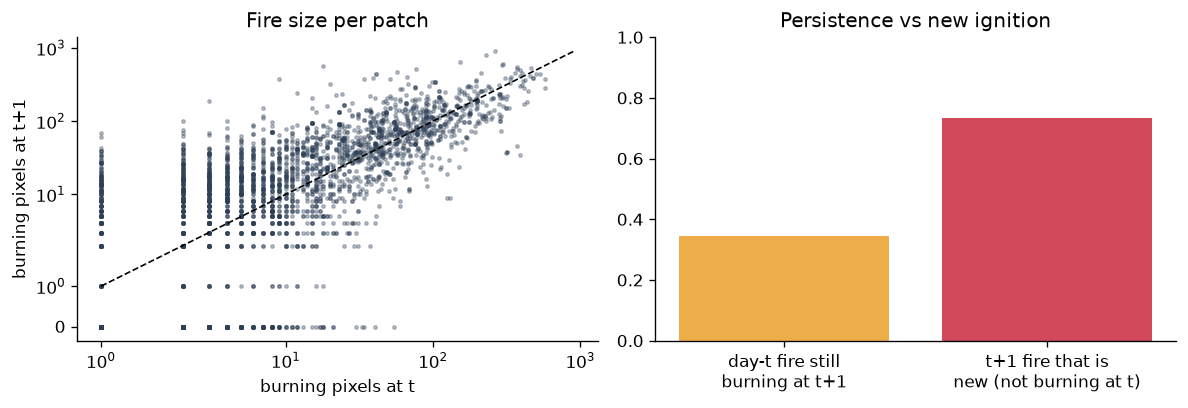
\includegraphics[width=\columnwidth]{eda/fire_dynamics.png}\\[2pt]
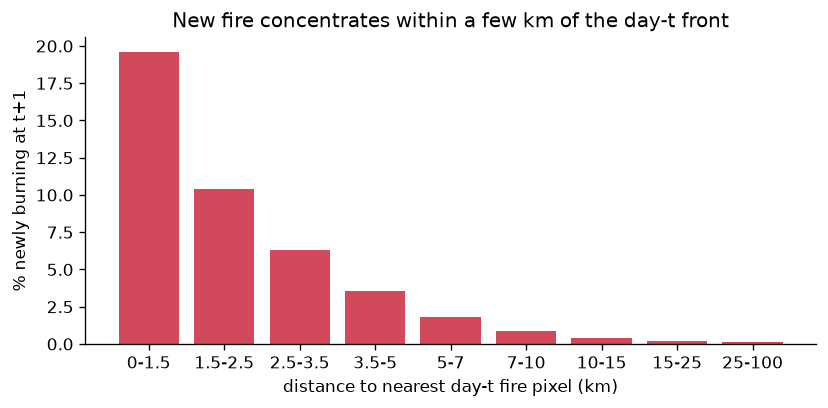
\includegraphics[width=0.49\columnwidth]{eda/spread_vs_distance.png}\hfill
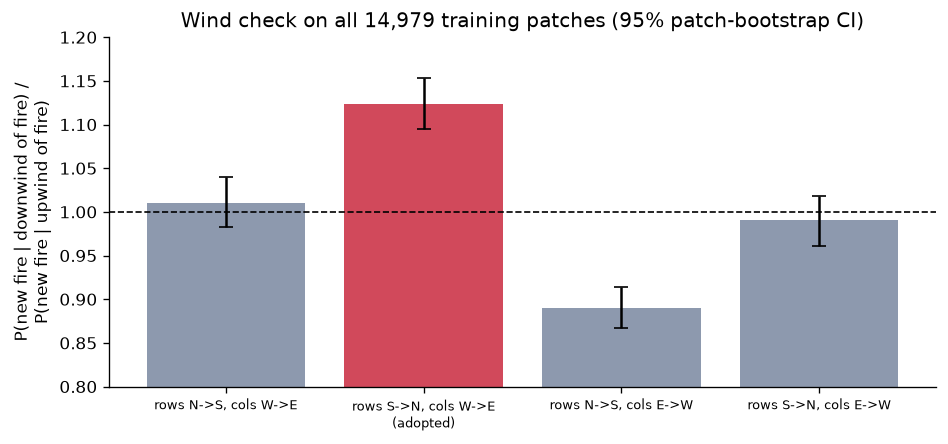
\includegraphics[width=0.49\columnwidth]{eda/wind_orientation.png}
\caption{How fire behaves in the data: how fire stays or moves (top), chance of fire by distance to today's fire (left), and the wind test used to find north (right).}
\label{fig:eda}
\end{figure}

\section{Feature Engineering}
A tree model sees one square at a time, so we give each square 32 features that describe its surroundings (Table~\ref{tab:features}). Every feature uses only today's data. For example, \emph{wind alignment} measures whether the wind is blowing from the nearest fire toward the square. Vapour-pressure deficit, a measure of how dry the air is, follows the FAO formula~\cite{allen1998fao56}.

\begin{table}[t]
\centering
\caption{The 32 tabular features}
\label{tab:features}
\footnotesize
\begin{tabular}{p{0.16\columnwidth}p{0.08\columnwidth}p{0.62\columnwidth}}
\toprule
Group & Count & Features \\
\midrule
Raw & 10 & elevation, wind speed, temperature min/max, humidity, rainfall, drought, NDVI, log population, ERC \\
Fire & 8 & today's fire and unknown flags, share of fire in windows of 3, 5, 9 and 17, distance to nearest fire, log fire count \\
Wind & 6 & east/north wind, fire up/downwind within 3 km, fire--wind alignment, wind push \\
Terrain & 4 & slope, aspect (sin, cos), upslope from fire \\
Weather & 2 & temperature range, vapour-pressure deficit \\
Vegetation & 2 & $5\times5$ NDVI mean and standard deviation \\
\bottomrule
\end{tabular}
\end{table}

\section{AML Methodology}
We use simple baselines: \emph{Dummy} (always predicts the average fire rate), \emph{persistence} (fire stays where it is) and neighbourhood persistence. We then train logistic regression, random forest, XGBoost and LightGBM.

Non-fire squares vastly outnumber fire squares, so training keeps every fire square and 2\% of the others. This makes the raw scores too high, so we correct them. With sampling rate $r$ and raw score $p_s$, the corrected probability~\cite{saerens2002prior} is
\begin{equation}
p = \frac{r\,p_s}{r\,p_s + 1 - p_s}.
\end{equation}
Boosted trees stop adding trees when validation performance stops improving, and we try a few tree sizes on validation data.

\section{Deep Learning Architecture}
Both networks produce a prediction for every square. The \emph{compact CNN} uses three blocks whose filters look further and further out, so each prediction sees a 29-square-wide area. It has \rCnnParameters{} parameters. The \emph{U-Net} first shrinks the map to capture the big picture, then expands it back to full size. \emph{Skip connections} carry fine detail straight across, so the edges of a fire stay sharp. It has \rUnetParameters{} parameters. Batch normalisation~\cite{ioffe2015batchnorm} and dropout~\cite{srivastava2014dropout} help training and reduce overfitting.

We train with weighted cross-entropy, which makes missing a fire more costly. With true label $y$, predicted chance $p$ and weight $w$, the loss is
\begin{equation}
\ell = -\left[w\,y\log p + (1-y)\log(1-p)\right].
\end{equation}
Training uses AdamW~\cite{loshchilov2019adamw}, stops early when validation performance stops improving, and flips and rotates images. It also uses random $32\times32$ crops, which hide the position of each patch's centre (Section~\ref{sec:leak}).

\section{Hybrid Methodology}
Hybrids try to combine the strengths of both approaches, because trees have useful hand-made features and networks can see shapes. We test two kinds:
\begin{itemize}
\item \emph{Feature-assisted U-Net:} the U-Net receives the hand-made features as extra inputs, for 31 input channels and \rUnetFeaturesParameters{} parameters.
\item \emph{Late fusion:} a small logistic regression learns how much to trust a tree and a network:
\begin{equation}
\operatorname{logit} p = a + b_1 \operatorname{logit} p_{\text{tree}} + b_2 \operatorname{logit} p_{\text{net}}.
\end{equation}
\end{itemize}
Here logit is the log of the odds of fire. Following stacking~\cite{wolpert1992stacking}, the weights are fitted on half of the validation data, which the base models did not train on. The other half chooses the best hybrid. Test data is never used for this choice.

\section{Experimental Setup}
\subsection{Three fair tests}
Elevation barely changes between days, so two patches with identical terrain are the same place. Using this, we grouped patches into \rLocationGroups{} locations. We found that about \rOfficialOverlap\% of the standard test patches share terrain with the training data. Table~\ref{tab:protocols} shows our three tests. A separate tuning split chooses the network settings, so no test patch influences them.

\begin{table}[t]
\centering
\caption{The three tests}
\label{tab:protocols}
\footnotesize
\begin{tabular}{lccc}
\toprule
Test & New weeks & New places & Train / val / test \\
\midrule
Official & Yes & No & \rOfficialTrain{} / \rOfficialVal{} / \rOfficialTest \\
Spatial & No & Yes & \rSpatialTrain{} / \rSpatialVal{} / \rSpatialTest \\
Strict & Yes & Yes & \rStrictTrain{} / \rStrictVal{} / \rStrictTest \\
\bottomrule
\end{tabular}
\end{table}

\subsection{Blocking the position shortcut}\label{sec:leak}
Every patch is centred on a fire. A model could learn that ``the middle burns'', which would not help in a real forecast~\cite{kayhan2020translation}. We use three protections: networks train on random crops; every model is also scored on fixed random windows where the centre is not special; and we measure the effect directly with a position-only predictor and a U-Net trained on full images.

\subsection{Tuning and repeats}
We tune one network setting at a time on the tuning split: model type, loss, dropout, weight decay, width and input channels. The final networks are trained three times with different random seeds. Hybrids use the first seed. Everything runs from one script, \texttt{scripts/run\_all.sh}, with settings in configuration files.

\subsection{Changes since Phase 1}
The graded Phase 1 materials remain unchanged on the \texttt{phase1-final-submission} branch. A full re-run reproduced the official and spatial scores to three decimals (Table~\ref{tab:phase1}). We made three additions: a strict split, because the Phase 1 spatial split still mixed weeks; a position-leak test, because Phase 1 did not test whether tabular models use position; and a Dummy baseline, CNN, tuned U-Net and hybrids.

\begin{table}[t]
\centering
\caption{Test PR-AUC at Phase 1 and in the final re-run}
\label{tab:phase1}
\scriptsize
\fitcolumn{tables/phase1_changes.tex}
\end{table}

\section{Evaluation Metrics}
Our main score is PR-AUC, computed on every known square. Random guessing scores about the fire rate, which differs between tests, so scores should be compared within a test. We also report recall at fixed false-alarm rates, confusion matrices, and other metrics in the Appendix. Table~\ref{tab:glossary} explains the terms used in this report.

\begin{table}[t]
\centering
\caption{Terms used in this report}
\label{tab:glossary}
\footnotesize
\begin{tabular}{p{0.26\columnwidth}p{0.64\columnwidth}}
\toprule
Term & Meaning \\
\midrule
Patch & One $64\times64$ km map of a fire \\
PR-AUC & How well a model finds real fires without too many false alarms; higher is better \\
Precision & When the model says fire, how often it is right \\
Recall & Of the real fires, how many the model finds \\
Lift & PR-AUC divided by the fire rate; how much better than random guessing \\
Leakage & When a model uses information it would not have in real use \\
95\% interval & A range showing how uncertain a score is, computed by resampling test patches 500 times \\
Paired test & Compares two models on the same resampled patches \\
Ablation & Removing one part to see how much it matters \\
\bottomrule
\end{tabular}
\end{table}

\section{Results}
\subsection{Main comparison}
Table~\ref{tab:summary} and Fig.~\ref{fig:comparison} give the main results. \textbf{The best tree model scored highest on all three tests.} Network rows use the first training seed; variation between seeds is covered below.

\begin{table}[t]
\centering
\caption{Test PR-AUC with 95\% intervals. Higher is better.}
\label{tab:summary}
\scriptsize
\fitcolumn{tables/results_summary.tex}
\end{table}

\begin{figure*}[t]
\centering
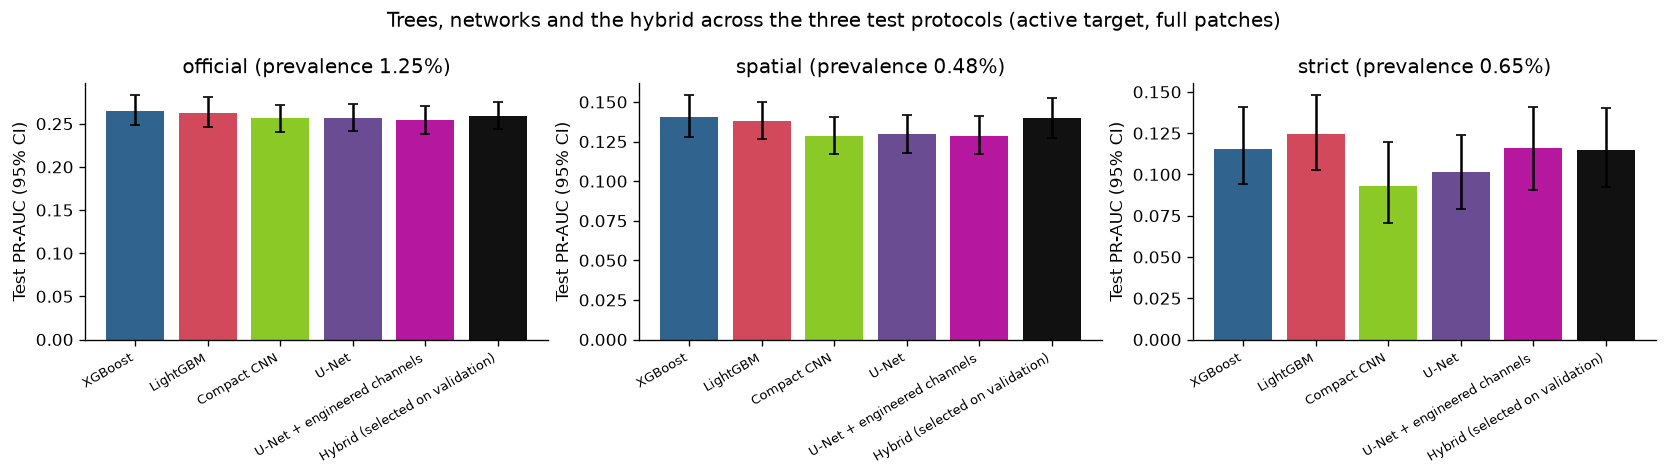
\includegraphics[width=0.92\textwidth]{final/model_comparison.png}
\caption{Test PR-AUC with 95\% intervals for the main models on each of the three tests.}
\label{fig:comparison}
\end{figure*}

\subsection{Are the differences real?}
The intervals in Table~\ref{tab:summary} overlap, so we use paired tests against XGBoost, the tree model chosen on validation data for all three tests. The U-Net is lower by \rOfficialFullActiveUnetMinusXgboostDelta, \rSpatialFullActiveUnetMinusXgboostDelta{} and \rStrictFullActiveUnetMinusXgboostDelta, and all three differences are statistically significant. So the networks' gap is small but real. LightGBM has the highest strict test score, but the paired test uses XGBoost because it was chosen on validation data. Full results are in Appendix Tables~\ref{tab:official}--\ref{tab:significance}.

\subsection{Scoring without the position shortcut}
On fixed random windows, position gives almost no information: a position-only predictor has a lift of just \rOfficialCropPositionPriorLift, \rSpatialCropPositionPriorLift{} and \rStrictCropPositionPriorLift. Here the gap narrows. On the official test the hybrid beats a window-trained LightGBM by \rOfficialCropActiveHybridMinusLightgbmCropDelta, which is the only significant hybrid win over a tree. On the spatial test the models are level. On the strict test the tree stays ahead of the U-Net by \rStrictCropActiveUnetMinusLightgbmCropDelta{} and of the hybrid by \rStrictCropActiveHybridMinusLightgbmCropDelta. Details are in Tables~\ref{tab:crop} and \ref{tab:sigcrop}.

\subsection{New fire only}
For squares not burning today (Table~\ref{tab:transition}), the U-Net beats XGBoost by \rOfficialFullTransitionUnetMinusXgboostDelta{} on the official test, but trails it by \rSpatialFullTransitionUnetMinusXgboostDelta{} and \rStrictFullTransitionUnetMinusXgboostDelta{} on the spatial and strict tests. The network's small lead does not carry over to places it has not seen.

\subsection{The position shortcut}
A predictor that uses only position scores \rOfficialFullCentrePriorPr, \rSpatialFullCentrePriorPr{} and \rStrictFullCentrePriorPr{} on full images. On the strict test it is higher than every valid model. A U-Net trained on full images gains \rOfficialFullActiveUnetFullpatchMinusUnetDelta, \rSpatialFullActiveUnetFullpatchMinusUnetDelta{} and \rStrictFullActiveUnetFullpatchMinusUnetDelta. We report these only as warnings, not as real results.

For tree models (Table~\ref{tab:leak}), adding position as a feature helps a lot, so our features do not already contain it. A separate model can partly recover closeness to the centre from the features (ROC-AUC \rOfficialLeakRecover, \rSpatialLeakRecover{} and \rStrictLeakRecover), most likely because fire itself is near the centre. Trees trained on full images and on windows score similarly, which suggests that the tree results do not depend on position.

\subsection{Hybrids}
The chosen hybrid was \rOfficialHybridSelected{} on the official and spatial tests and \rStrictHybridSelected{} on the strict test (Table~\ref{tab:fusion}). It was \rOfficialFullActiveHybridMinusXgboostDelta{} below XGBoost on the official test, which is significant, and level with it on the other two (\rSpatialFullActiveHybridMinusXgboostDelta{} and \rStrictFullActiveHybridMinusXgboostDelta, with intervals containing zero). It beat the U-Net on the two harder tests. So the hybrid improves the network but not the trees.

\subsection{Different training seeds}
Table~\ref{tab:seeds} repeats training three times. Scores vary by a standard deviation of \rSeedSdMin{} to \rSeedSdMax, which is similar to several gaps between models. Adding features to the U-Net gave the largest gain on the strict test (mean \rStrictUnetFeaturesSeedMean{} against \rStrictUnetSeedMean), but it also varied the most, so we treat it as a hint rather than a proven gain.

\subsection{Maps and errors}
Fig.~\ref{fig:example} shows one example. Models work well near today's fire and miss fire that moves further away. XGBoost finds \rOfficialRecallNear, \rSpatialRecallNear{} and \rStrictRecallNear{} of fire within 1.5 km of today's fire on the three tests, but only \rOfficialRecallMid, \rSpatialRecallMid{} and \rStrictRecallMid{} between 1.5 and 3.5 km, and almost none beyond that. More examples are in Fig.~\ref{fig:maps} and Fig.~\ref{fig:errors}.

\begin{figure}[t]
\centering
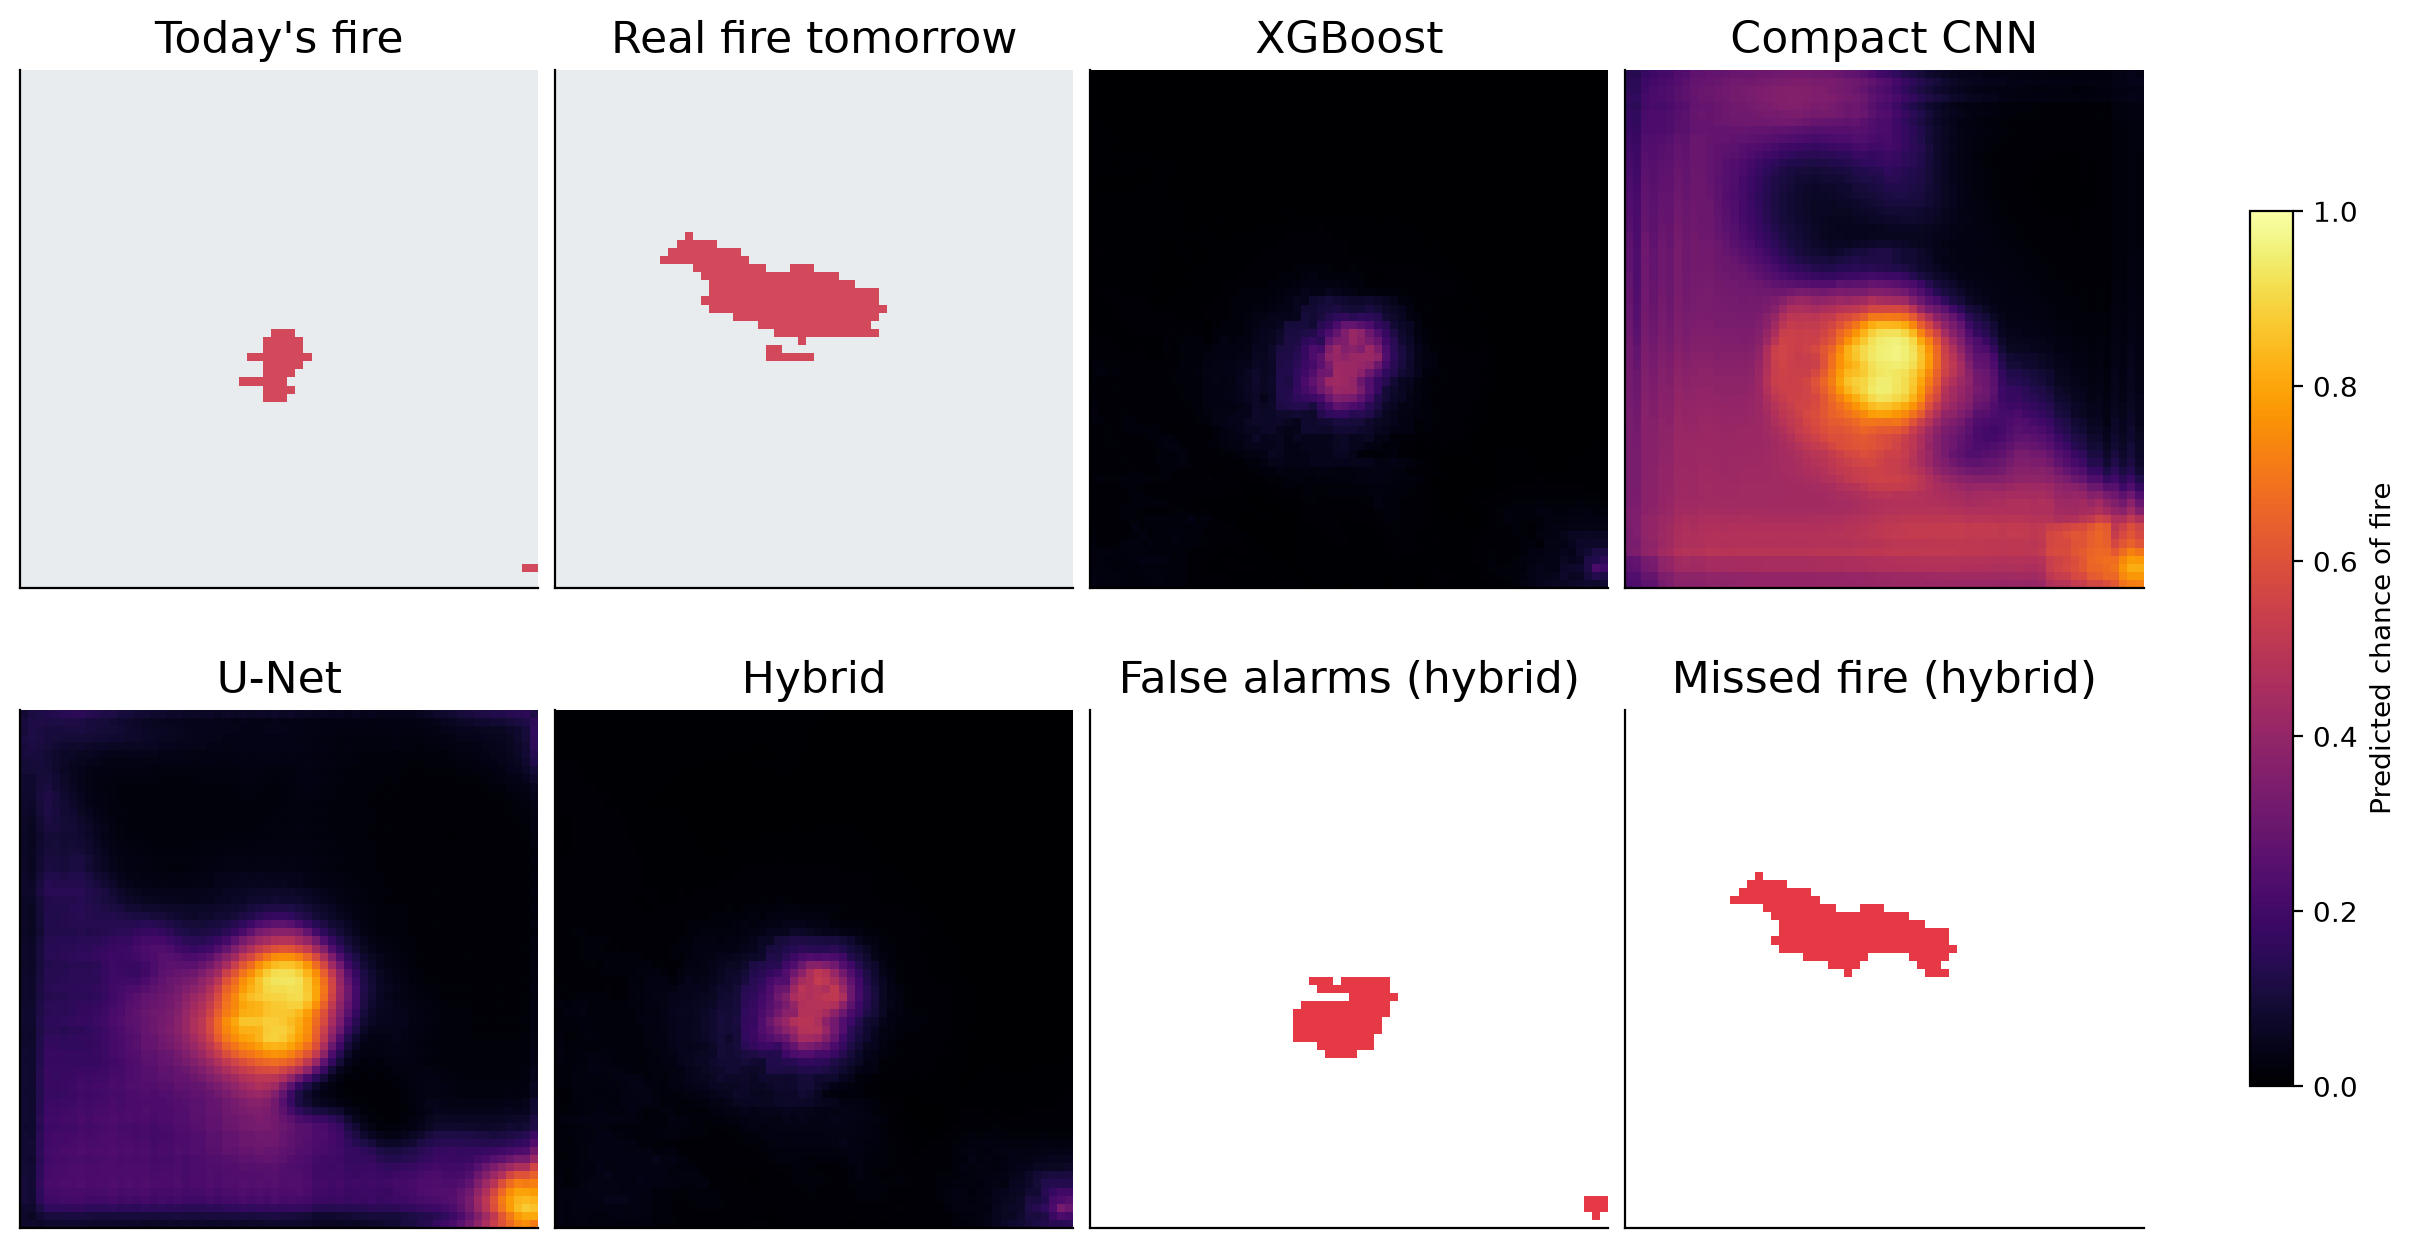
\includegraphics[width=\columnwidth]{final/strict/prediction_map_example.png}
\caption{One strict-test example, showing today's fire, tomorrow's real fire, each model's predicted chance of fire, and the hybrid's false alarms and missed fire.}
\label{fig:example}
\end{figure}

\section{Ablation Studies}
An ablation removes one part to see how much it matters. Table~\ref{tab:dlablation} and Fig.~\ref{fig:dlablation} show the U-Net results. \textbf{Removing today's fire map drops the score from \rAblationBaseline{} to \rAblationNoPrevFireChannel.} Other removals changed it only slightly: no skip connections gave \rAblationNoSkipConnections, no weather gave \rAblationNoWeatherChannels{} and no wind gave \rAblationNoWindChannels. Removing image flips gave \rAblationNoAugmentation, slightly above the chosen model, so we do not claim that augmentation helped. Each is a single run, so small differences should not be over-read.

For tree models (Table~\ref{tab:tabularablation}), raw values alone are weak (\rSpatialTabularRawOnly{} on spatial and \rStrictTabularRawOnly{} on strict), and fire features alone reach \rSpatialTabularFireOnly{} and \rStrictTabularFireOnly.

\begin{table}[t]
\centering
\caption{U-Net ablations on the tuning split}
\label{tab:dlablation}
\scriptsize
\fitcolumn{tables/dl_ablations.tex}
\end{table}

\begin{figure}[t]
\centering
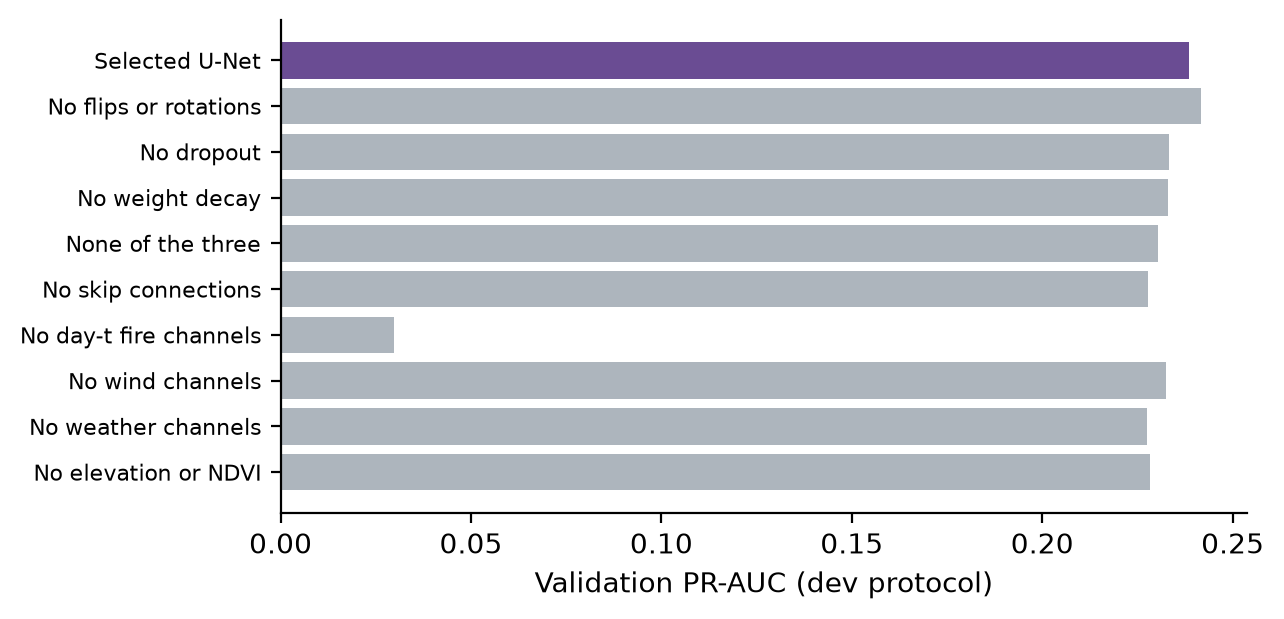
\includegraphics[width=\columnwidth]{final/dl_ablations.png}
\caption{Effect of each ablation on the U-Net's validation PR-AUC.}
\label{fig:dlablation}
\end{figure}

\section{Discussion}
\emph{Why did trees stay ahead?} The ablations show that tomorrow's fire depends mostly on today's fire and its immediate surroundings, and our features describe exactly that. Networks can learn these patterns too, but only have about $10^4$ patches to learn from. This agrees with Grinsztajn et al.~\cite{grinsztajn2022tabular}, although we did not test this explanation directly.

\emph{How much does the test matter?} Moving from the official test to tests on new places roughly halves PR-AUC, partly because fire is rarer in those tests. Trees stay ahead of networks in the full-image scores, so shared terrain does not explain their lead.

\emph{Position.} Full-image scores include a large position effect, so scores from different studies can only be compared when they handle position in the same way. Our scores are also not directly comparable with published NDWS scores, because training and evaluation details differ.

\emph{Hybrids.} Combining a tree and a network improved on the network in the two harder tests, but did not beat the best tree.

\emph{In practice,} models mostly find fire next to today's fire and rarely detect spread several kilometres away.

\section{Limitations}
\begin{itemize}
\item NDWS has no coordinates, dates, fire names, fuel moisture or firefighting information.
\item Weeks are assigned at random, so we test new weeks but not future seasons.
\item Weather covers all of today, so a forecast can only be issued after the day ends.
\item Satellite fire labels can be wrong because of cloud, smoke and timing.
\item We can only detect exactly matching terrain, so nearby fires may appear in both training and test data.
\item The strict test has only \rStrictTest{} patches, so its results are uncertain.
\item Every sample contains a fire, so results do not apply to monitoring all land.
\item Tuning and ablation results come from single runs.
\end{itemize}

\section{Conclusion}
Tree models with well-designed features were the strongest models on all three tests. The CNN, U-Net and hybrids came close but did not beat them. The hybrid improved on the U-Net on the two harder tests and did not beat the best tree, so the hybrid idea was tested and not supported as an improvement over trees. The strict test and the position tests show that scores depend strongly on how data is split and sampled.

\section{Future Work}
Useful next steps are to use WildfireSpreadTS~\cite{gerard2023wildfirespreadts}, which has real dates and fire names; to try models that use several days, such as ConvLSTM~\cite{shi2015convlstm}; to add fuel-moisture data; and to make the predicted probabilities more reliable for operational use.

\section*{Reproducibility and Contributions}
All code, settings and results are in the project repository. \texttt{scripts/run\_all.sh} reproduces every experiment, and every number here is generated from the result files. Individual contributions are in \texttt{CONTRIBUTIONS.md}.

\appendices
\section{Detailed Results}
These tables and figures give the full detail behind the results in the main text.

\begin{table*}[t]
\centering
\caption{Official test (new weeks), active target, full images. Thresholded metrics use validation thresholds.}
\label{tab:official}
\footnotesize
\fitwide{tables/results_official_full.tex}
\end{table*}

\begin{table*}[t]
\centering
\caption{Spatial test (new places), active target, full images.}
\label{tab:spatial}
\footnotesize
\fitwide{tables/results_spatial_full.tex}
\end{table*}

\begin{table*}[t]
\centering
\caption{Strict test (new weeks and places), active target, full images.}
\label{tab:strict}
\footnotesize
\fitwide{tables/results_strict_full.tex}
\end{table*}

\begin{table}[t]
\centering
\caption{Paired differences in test PR-AUC, full images (first seed).}
\label{tab:significance}
\scriptsize
\fitcolumn{tables/significance.tex}
\end{table}

\begin{table}[t]
\centering
\caption{Test results on fixed $32\times32$ windows.}
\label{tab:crop}
\scriptsize
\textbf{Official}\\[2pt]\fitcolumn{tables/results_official_crop.tex}\\[6pt]
\textbf{Spatial}\\[2pt]\fitcolumn{tables/results_spatial_crop.tex}\\[6pt]
\textbf{Strict}\\[2pt]\fitcolumn{tables/results_strict_crop.tex}
\end{table}

\begin{table}[t]
\centering
\caption{Paired differences on fixed windows (first seed).}
\label{tab:sigcrop}
\scriptsize
\fitcolumn{tables/significance_crop.tex}
\end{table}

\begin{table}[t]
\centering
\caption{PR-AUC on the transition target (new fire only).}
\label{tab:transition}
\scriptsize
\fitcolumn{tables/results_transition.tex}
\end{table}

\begin{table}[t]
\centering
\caption{Position-leak tests of LightGBM on test data.}
\label{tab:leak}
\scriptsize
\fitcolumn{tables/leak_test.tex}
\end{table}

\begin{table*}[t]
\centering
\caption{Hybrid candidates. Weights are fitted on half of validation data, and the other half selects the hybrid.}
\label{tab:fusion}
\footnotesize
\fitwide{tables/fusion.tex}
\end{table*}

\begin{table}[t]
\centering
\caption{Test PR-AUC across three training seeds.}
\label{tab:seeds}
\scriptsize
\fitcolumn{tables/seed_stability.tex}
\end{table}

\begin{table}[t]
\centering
\caption{LightGBM feature-group ablations, PR-AUC.}
\label{tab:tabularablation}
\scriptsize
\fitcolumn{tables/tabular_ablations.tex}
\end{table}

\begin{table}[t]
\centering
\caption{Hyperparameter sweep on the tuning split, validation PR-AUC.}
\label{tab:sweep}
\scriptsize
\fitcolumn{tables/sweep.tex}
\end{table}

\begin{figure*}[t]
\centering
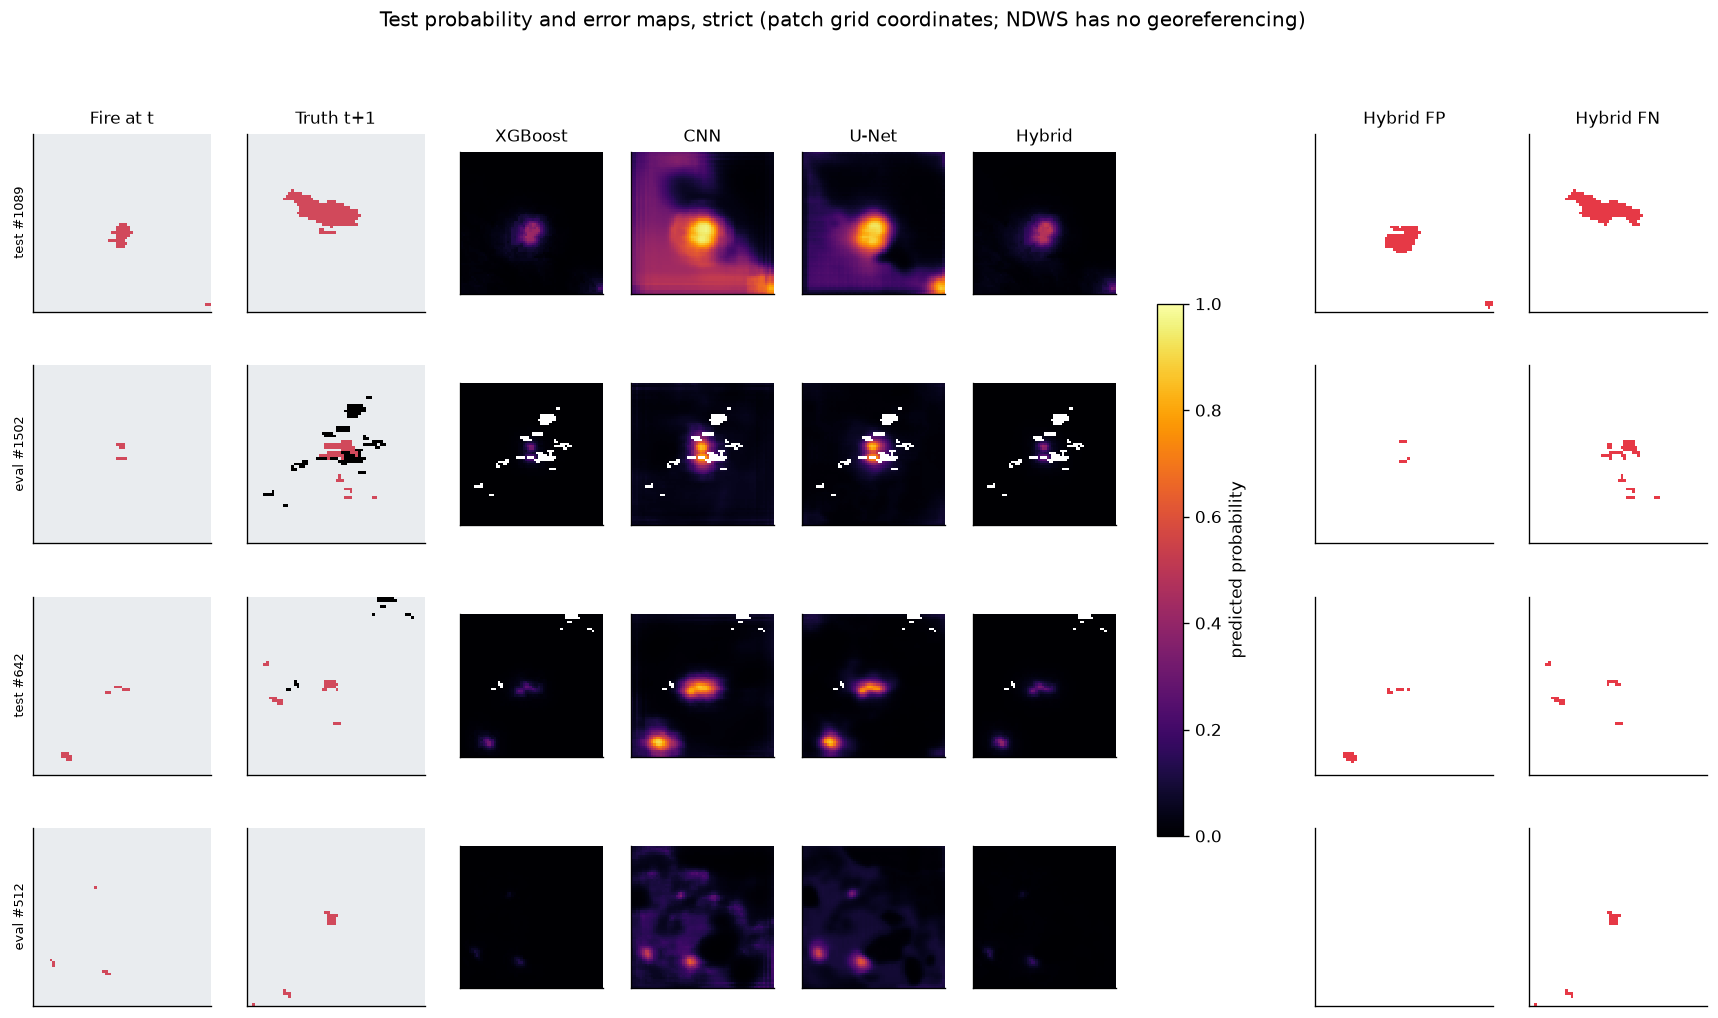
\includegraphics[width=0.95\textwidth]{final/strict/prediction_maps.png}
\caption{More strict-test maps: today's fire, tomorrow's real fire, XGBoost, CNN, U-Net, hybrid, and hybrid false alarms and misses. Axes are grid positions because NDWS has no coordinates.}
\label{fig:maps}
\end{figure*}

\begin{figure}[t]
\centering
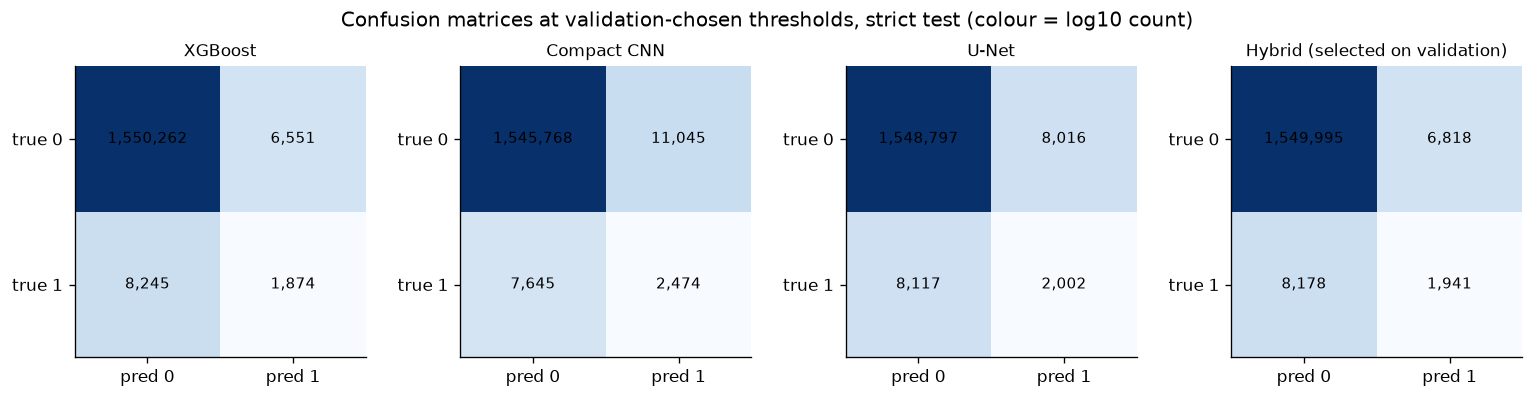
\includegraphics[width=\columnwidth]{final/strict/confusion_matrices.png}\\[3pt]
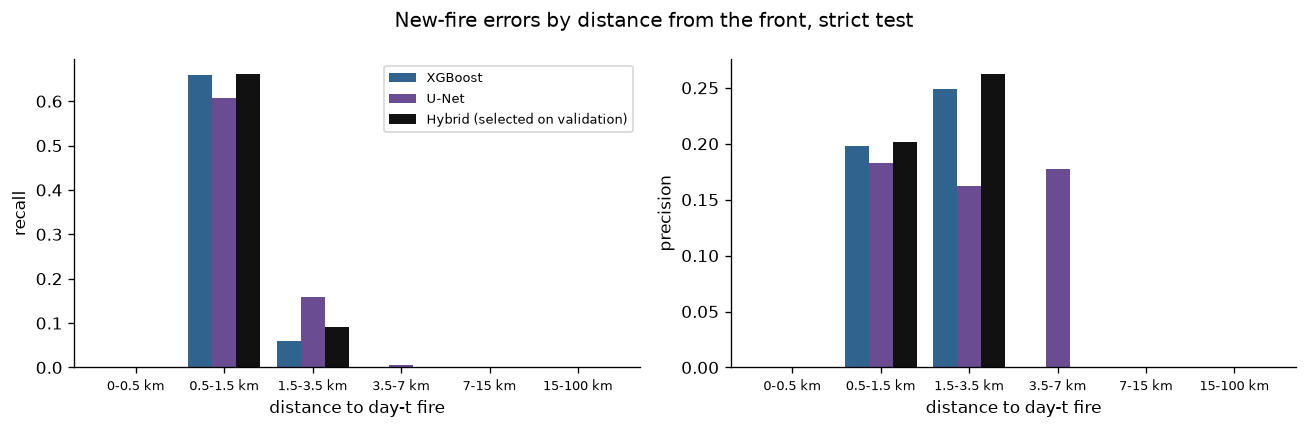
\includegraphics[width=\columnwidth]{final/strict/error_by_distance.png}
\caption{Strict-test confusion matrices (top) and errors by distance to today's fire (bottom).}
\label{fig:errors}
\end{figure}

\clearpage
\bibliographystyle{IEEEtran}
\bibliography{references}

\end{document}
